\chapter{Reinforcement Learning} \label{ch:ch2}

Reinforcement learning (RL) is a field of machine learning that is experiencing a period of great fervour in the world of research, fomented by recent progress in deep learning (DL) which opened the doors to function approximation developing what is nowadays known as deep reinforcement learning.
RL represents the third paradigm of machine learning alongside supervised and unsupervised learning.
The idea underlying this research field is that the learning process to solve a decision-making problem consists in a sequence of trial and error where the \textit{agent}, the protagonist of RL, could discover and discriminate valuable decisions from penalising ones exploiting information given by a \textit{reward signal}.
This interaction has a strong correlation with what human beings and animals do in the real world to forge their behaviour.

Before discussing the results of this thesis, it is good to delineate what today represents the state-of-the-art to understand the universe behind this paradigm better.
Indeed, the exploration of this field of research is the main aim of this chapter: the first section begins with the definition of the notation used and with the theoretical foundations behind traditional RL, then in the second section it moves progressively towards what is deep RL through an introduction to the fundamentals of deep learning and a careful discussion of the most essential algorithms paying more attention to those used during the thesis project.
The last section aims to illustrate the starting point and ideas of the thesis, drawing what the scenario of deep RL applied to autonomous systems and real-world robotic tasks is today.

The elaboration of this chapter is inspired by \cite{silver2015lectures}, \cite{sutton2018reinforcement}, \cite{openai2018spinningup}, \cite{lapan2018deep} and \cite{franccois2018introduction}.

\section{Fundamentals of reinforcement learning} \label{fundreinflearn}

Reinforcement learning is a computational approach to sequential decision making.
It provides a framework that is exploitable with decision-making problems that are unsolvable with a single action and need a sequence of actions, a broader horizon, to be solved.
This section aims to present the fundamental ideas and notions behind this research field in order to help the reader to develop a baseline useful to approach \vref{deepreinflearn} about deep reinforcement learning.

\subsection{The reinforcement learning problem}

\subsubsection{Agent, environment and reward}

The primary purpose of RL algorithms is to learn how to improve and maximise a future reward by relying on interactions between two main components: the \textit{agent} and the \textit{environment}.

The \textit{agent} is the entity that interacts with the environment by making decisions based on what it can observe from the state of the surrounding situation. The decisions taken by the agent consist of \textit{actions} ($a_t$).  The agent has no control over the environment, but actions are the only means by which it can modify and influence the environment.
Usually, the agent has a set of actions it can take, which is called \textit{action space}.
Some environments have \textit{discrete} action spaces, where only a finite number of moves are available (e.g. $\mathcal{A} = [\text{North}, \text{South}, \text{East}, \text{West}]$ choosing the direction to take in a bidimensional maze). On the other side, there are \textit{continuous} action spaces where actions are vectors of real values.
This distinction is fundamental to choose the right algorithm to use because not all of them could be compatible with both types: according to the needs of the specific case, it may be necessary to modify the algorithm to make it compatible. The sequence of states and actions is named \textit{trajectory} ($\tau$): it is helpful to represent an episode in the RL framework.

The \textit{environment ($E$)} represents all the things that are outside the agent. Whenever the agent takes an action, it emits a \textit{reward} and an \textit{observation} of the environment.

The \textit{reward} $r_t$ is a scalar feedback signal that defines the objective of the RL problem. This signal allows the agent to be able to distinguish positive actions from negative ones in order to reinforce and improve its behaviour. It is crucial to notice that the reward is local: it describes only the value of the latest action. Furthermore, actions may have long term consequences, delaying the reward. As it happens with human beings' decisions, receiving a conspicuous reward at a specific time step does not exclude the possibility to receive a small reward immediately afterwards and sometimes it may be better to sacrifice immediate reward to gain greater rewards later.

In this context, many features make reinforcement learning different from supervised and unsupervised learning.
Firstly, there is no supervisor: when the agent has to decide what action to take, there is no entity that can determine what the optimal decision is in that specific moment. It does not learn from a set of labelled objects taken from a knowledge base as in supervised learning, but it exploits its direct experience composed by observations and rewards as a feedback. On the other hand, the presence of a mapping between input and output is the main difference from unsupervised learning, where the objective is to find underlying patterns rather than mappings.

The agent receives only a reward signal which may delay compared to the moment in which it has to perform the next action. This fact brings out another significant difference: the importance of time. The sequentiality links all actions taken by the agent, making resulting data no more independent and identically distributed (i.i.d).

\subsubsection{The concept of return}

Given these definitions, it is noticeable that the primary purpose of the agent is to maximise the cumulative reward called \textit{return}.


The \textit{return $g_t$} is the total discounted reward starting from timestep $t$ defined by \vref{eq:return} where $\gamma$ is a \textit{discount factor}.
\begin{equation} \label{eq:return}
	g_t = r_{t+1} + \gamma r_{t+2} + \dots = \sum_{k=0}^{\infty} \gamma^k r_{t+k+1}, \;\;\;\gamma \in [0,1)
\end{equation}
Not only the fact that animal and human behaviour show a preference for immediate rewards rather than for the future ones motivates the presence of this factor, but it is also mathematically necessary: an infinite-horizon sum of rewards may not converge to a finite value. Indeed, the return function is a geometric series, so, if $\gamma \in [0,1)$, the series converges to a finite value equal to $1/(1-\gamma)$. For the same convergence sake, the case with $\gamma = 1$ makes sense only with a finite-horizon cumulative discounted reward.

\subsubsection{States and observations}

The other data emitted by the environment is the \textit{observation} ($o_t$) that is related to the \textit{state} ($s_t$). It represents a summary of information that the agent uses to select the next action, while the \textit{state} is a function of the \textit{history}, the sequence of observation, actions and rewards at timestep $t$ as shown in \vref{eq:history}.
\begin{equation}\label{eq:history}
	h_t = o_1, r_1, a_1, \dots, a_{t-1}, o_{t}, r_t, \;\;\;\;\; s_t = f(h_t)
\end{equation}
The state described above is also called \textit{agent state} $s_t^a$, while the private state of the environment is called \textit{environment state} $s_t^e$. This distinction is useful for distinguishing fully observable environments where $o_t = s_t^e = s_t^a$, from partially observable environments where $s_t^e \neq s_t^a$.
In the first case, the agent can observe the environment state directly, while in the second one, it has access to partial information about the state of the environment.
Beyond the fact that this chapter will focus on fully observable environments, the distinction between state and observation is often unclear and, conventionally, the input of the agent is composed by the reward and the state as shown in \vref{fig:interactionsAE}.

Furthermore, a state is called \textit{informational state} (or \textit{Markov state}) when it contains all data and information about its history. Formally, a state is a Markov state if and only if satisfies \vref{eq:markov_state}.
\begin{equation} \label{eq:markov_state}
	\mathbb{P}[s_{t+1}| s_t] = \mathbb{P}[s_{t+1} | s_1, \dots, s_t]
\end{equation}
It means that the state contains all data and information the agent needs to know to make decisions: the whole history is not useful anymore because it is inside the state. The environment state $s_t^e$ is a Markov state.

\begin{figure}
	\centering
	\begin{tikzpicture}
		% node Agent
		\node[punkt] (agent) {Agent};
		% node Environment
		\node[punkt, below=2cm of agent] (env) {Environment};
		% node a_t
		\node[mylabel, below right=0.75cm and 0cm of agent] (action) {$a_t$};
		% node s_t
		\node[mylabel, below left=0.75cm and 0.8cm of agent] (state) {$s_t$};
		% node r_t
		\node[mylabel, below left=0.75cm and -0.3cm of agent] (reward) {$r_t$};
		% node s_t+1
		\node[mylabel, above left=-1.3cm and -1cm of env] (state) {$s_{t+1}$};
		% node r_t+1
		\node[mylabel,above left=-.3cm and -1cm of env] (reward1) {$r_{t+1}$};
		\draw[pil]   (agent.east) -- ($(agent.east) + (1.2cm,0cm)$)  |-  (env.east);
		\draw[pil]   ($(env.west) + (0,-0.2cm)$) -- ($(env.west) + (-1.2cm,-0.2cm)$);
		\draw[pil]   ($(env.west) + (-1.2cm,-0.2cm)$) -- ($(env.west) + (-2cm,-0.2cm)$) |-($(agent.west) + (0,0.2cm)$);
		\draw[pil]   ($(env.west) + (0,+0.2cm)$) -- ($(env.west) + (-1.2cm,+0.2cm)$);
		\draw[pil]   ($(env.west) + (-1.2cm,+0.2cm)$) -- ($(env.west) + (-1.6cm,+0.2cm)$) |-($(agent.west) + (0,-0.2cm)$);
		\draw[dashed]  ($(env.west) - (1.2cm,-0.5cm)$) -- ($(env.west) - (1.2cm,0.5cm)$);
	\end{tikzpicture}
	\caption[Interaction loop between Agent and Environment]{Interaction loop between Agent and Environment. The reward and the state resulting from taking an action become the input of the next iteration. \cite{sutton2018reinforcement}}
	\label{fig:interactionsAE}
\end{figure}
\subsubsection{The Markov decision problem}

With all the definitions shown so far, it is possible to formalise the type of problems on which RL can unleash all its features: the Markov decision process (MDP), a mathematic framework to model decision processes. Its main application fields are optimisation and dynamic programming.

A MDP is defined by:
\begin{equation}\label{eq:mdp}
	\begin{gathered}
		<\mathcal{S}, \mathcal{A}, \mathcal{P}, \mathcal{R}, \gamma>\\
		\begin{aligned}
			\text{where}\hspace{10pt} \mathcal{S} & \text{ is a finite set of states}                     \\
			\mathcal{A}                           & \text{ a finite set of actions}                       \\
			\mathcal{P}                           & \text{ a state transition probability matrix}\;\;
			\mathcal{P}_{ss'}^a = \mathbb{P}[s_{t+1}= s' | s_t = s, a_t = a]                              \\
			\mathcal{R}                           & \text{ a reward function}
			\;\; \mathcal{R}_{s}^a = \mathbb{E}[r_{t+1} | s_t = s, a_t = a]                               \\
			\gamma                                & \text{ a discount factor such that } \gamma \in [0,1]
		\end{aligned}
	\end{gathered}
\end{equation}
The main goal of an MDP is to select the best action to take, given a state, in order to collect the best reward achievable.

\subsubsection{Policies, models and value functions} \label{pmvf}
The components that may compose the agent, the brain of the reinforcement learning problem, can not be missing: they are the \textit{model}, the \textit{policy} and the \textit{value function}.

A \textit{model} consist of information about the environment. These data must not be confused with the ones provided by states and observations: they make it possible to infer prior knowledge about the environment, influencing the behaviour of the agent.

A \textit{policy} is the representation of the agent's behaviour. It is a function that describes the mapping from states to actions.  The policy is represented by $\pi$ and it may be deterministic  $a_t = \pi(s_t)$  or stochastic $\pi(a_t|s_t) = \mathbb{P}[a_t | s_t]$.
In this perspective, it is evident that the central goal of RL is to learn an optimal policy $\pi^*$. The optimal policy is a policy which can show to the agent what the most profitable way to achieve the maximum return is, what is the best action to do in a specific situation. In order to learn the nature of the optimal policy, RL exploits value functions.

A \textit{value function} represents what is the expected reward that the agent can presume to collect in the future, starting from the current state. The reward signal represents only a local value of the reward, while the value function provides a broader view of future rewards: it is a sort of prediction of rewards.
It is possible to delineate two main value functions: the \textit{state value} function and the \textit{action value} function.

\begin{itemize}
	\item The \textit{State Value Function} $V^\pi(s)$ is the expected return starting from the state $s$ and always acting according to policy $\pi$.
	      \begin{equation} \label{eq:statevalue}
		      V^\pi(s) = \mathbb{E}_{\tau \sim \pi}[g_t | s_0 = s]
	      \end{equation}
	\item The \textit{Action Value Function} $Q^\pi(s)$ is the expected return starting from the state $s$, taking an action $a$ and then always acting according to policy $\pi$.
	      \begin{equation} \label{eq:actionvalue}
		      Q^\pi(s, a) = \mathbb{E}_{\tau \sim \pi}[g_t | s_0 = s, a_0 = a]
	      \end{equation}
\end{itemize}


\subsection{Bellman equations}

Both \vref{eq:statevalue,eq:actionvalue} satisfy recursive relationships between the value of a state and the values of its successor states. It is possible to see this property deriving \textit{Bellman equations} \cite{bellman2015applied} -- shown in \vref{eq:bellman} and demonstrated in \vref{appendix:bellmaneq} -- where $s_{t+1}\sim \mathit{E}$ means that the next state is sampled from the environment $E$ and $a_{t+1}\sim \pi$ shows that the policy $\pi$ determines the next action.
\begin{align} \label{eq:bellman}
	\begin{split}
		V^\pi(s_t) &= \mathbb{E}_{a_t \sim \pi, s_{t+1} \sim E}[r(s_t, a_t) + \gamma V^\pi(s_{t+1})] \\
		&= \sum_{a \in \mathcal{A}}\pi(a|s)\sum_{s' \in \mathcal{S}, r \in \mathcal{R}}P(s', r | s, a)\big[r + \gamma V^\pi(s')\big]\\
		Q^\pi(s_t,a_t) &= \mathbb{E}_{s_{t+1} \sim E}[r(s_t, a_t) + \gamma \mathbb{E}_{ a_{t+1} \sim \pi}[Q^\pi(s_{t+1}, a_{t+1})]]\\
		&= \sum_{a \in \mathcal{A}}\pi(a|s)\sum_{s' \in \mathcal{S}, r \in \mathcal{R}}P(s', r | s, a)\big[r + \gamma Q^\pi(s',a')\big]\\
	\end{split}
\end{align}
$r(s_t, a_t)$ is a placeholder function to represent the reward given the starting state and the action taken.
As discussed above, the goal is to find the optimal policy $\pi^*$ to exploit. It can be done using \textit{Bellman optimality equations} defined in \vref{eq:optbellman}.
\begin{align} \label{eq:optbellman}
	\begin{split}
		V^*(s_t) &= \max_{a} \mathbb{E}_{s_{t+1} \sim E}[r(s_t, a) + \gamma V^*(s_{t+1})] \\
		&= \max_{a}\sum_{s' \in \mathcal{S}, r \in \mathcal{R}}P(s', r | s, a)\big[r + \gamma V^*(s')\big]\\
		Q^*(s_t,a_t) &= \mathbb{E}_{s_{t+1} \sim E}[r(s_t, a_t) + \gamma \max_{a'}[Q^*(s_{t+1}, a')]]\\
		&= \sum_{s' \in \mathcal{S}, r \in \mathcal{R}}P(s', r | s, a)\big[r + \gamma \max_{a'} Q^*(s',a')\big]\\
	\end{split}
\end{align}

Therefore, value functions allow defining a partial ordering over policies such that \[\pi \ge \pi' \text{ if } V_\pi \ge V_{\pi'},\forall s \in \mathcal{S}\]
This definition is helpful to enounce the \textit{sanity theorem}. It asserts that for any MDP there exists an optimal policy $\pi^*$ that is better than or equal to all other policies, $\pi^* \ge \pi, \forall \pi$, but also that all optimal policies achieve the optimal state value function and the optimal action-value function.

The solution of the Bellman optimality equation is not linear and, in general, there is no closed-form solution. For this reason, there are many iterative methods: \vref{dp,mfa} contain some of them.


\subsection{Approaches to Reinforcement Learning} \label{approaches}

Every agent consists of an RL algorithm that it exploits to maximise the reward it receives from the environment. Every single algorithm has its singularity, and it could work with a specific application field which depends on the particular approach it supports. Understanding differences among these groups is useful to adequately understand what type of algorithm satisfies better the needs of a specific problem. Nowadays, RL algorithms are numerous, and drawing the complete picture behind them could be a complicated purpose. The distinctions presented in this section aims to describe the most crucial distinctions that are useful in the context of the thesis without claiming to be exhaustive.

\subsubsection{Components of learning}

The first worthy distinction between RL algorithms can be made analysing how the algorithms exploit the different components of the agent: indeed it is possible to explain the main strategies in RL using \textit{policy}, \textit{model} and \textit{value function} defined in \vref{pmvf}.


One of the most crucial aspects of an RL algorithm is the question of whether the agent has access to or learns the model of the environment: this element enables the agent to predict state transitions and rewards.
A method is \textit{model-free} when it does not exploit the model of the environment to solve the problem. All the actions made by the agent results from direct observation of the current situation in which the agent is. It takes the observation, does computations on them and then select the best action to take.
This last representation is in contrast with \textit{model-based} methods. In this case, the agent tries to build a model of the surrounding environment in order to infer information useful to predict what the next observation or reward would be.
Both groups of methods have strong and weak sides.
Ordinarily, \textit{model-based} methods show their potential in a deterministic environment (e.g. board game with rules). In these contexts, the presence of the model enables the agent to plan by reasoning ahead, to recognise what would be the result of a specific decision before acting. The agent can extract all this knowledge and learn an optimal policy to follow. However, this opportunity is not always achievable: the model may be partially or entirely unavailable, and the agent would have to learn the model from its experience. Learning a model is radically complex and may lead to various hurdles to overcome: for instance, the agent can exploit the bias present in the model, producing an agent which is not able to generalise in real environments.
On the other hand, model-free methods tend to be more straightforward to train and tune because it is usually hard to build models of a heterogeneous environment. Furthermore, model-free methods are more popular and have been more extensively developed and tested than model-based methods.

The use of policy or value function as the central part of the method represents another essential distinction between RL algorithms.
The approximation of the policy of the agent is the base of \textit{policy-based} methods. The representation of the policy is usually a probability distribution over available actions. This method points to optimise the behaviour of the agent directly and may ask manifold observations from the environment: this fact makes this method not so sample-efficient.
On the opposite side, methods could be \textit{value-based}. In this case, the agent is still involved in finding the optimal behaviour to follow, but indirectly. It is not interested anymore about the probability distribution of actions. Its main objective is to determine the value of all actions available, choosing the best one. The main difference from the policy-based method is that this method can benefit from other sources, such as old policy data or replay buffer.

\begin{figure}
	\centering
	\begin{tikzpicture}
		% node Agent
		\node[punkt] (experience) {Experience};
		% node Environment
		\node[punkt, below left=0.75cm and 0.75cm of experience] (model) {Model};
		% node Value/Policy
		\node[punkt, below right=0.75cm and 0.75cm of experience] (valpol) {Value/Policy};
		\node[mylabel, above left=0.05cm and 0.00cm of experience.west] (ml) {\footnotesize Model learning};
		\node[mylabel, above right=0.05cm and 0.3cm of experience.east] (a) {\footnotesize Acting};
		\node[mylabel, below right=0.5cm and -0.3cm of experience.south] (a) {\footnotesize Model-Free};
		\node[mylabel, above right=-0.2cm and -0.5cm of model.east] (a) {\footnotesize Planning};
		\draw[pil]   (experience.south) -- ($(experience.south) - (0cm,1cm)$)  |-  ($(valpol.west) + (0cm,0.2cm)$);
		\draw[pil]   (experience.west)  -| (model.north);
		\draw[pil]   (valpol.north) -- ($(valpol.north) + (0cm,1cm)$)  |-  (experience.east);
		\draw[pil]   ($(model.east) - (0cm,0.2cm)$)  --  ($(valpol.west) - (0cm,0.2cm)$);
	\end{tikzpicture}
	\caption[Overview of different components in reinforcement learning]{ Overview of components of an agent with their relation in respect of different approaches of learning. Model-Free methods works with the experience, value functions and the policy, while model-based techniques tries to build up a model to derive value functions and policy to act in the environment.}
	\label{fig:components}
\end{figure}

\subsubsection{Learning settings}

The learning setting could be \textit{online} or \textit{offline}. In the first case, the learning process is done in parallel or concurrently while the agent continues to gather new information to use, while the second one progresses toward learning using limited data.
Generalisation becomes a critical problem in the latter approach because the agent is not able to interact anymore with the environment.
In the context of this thesis, what matters is \textit{online learning}: the learning phase is not bound to already gathered data, but the whole process goes on using both old data coming from replay buffers and brand new data obtained in the most recent episode.

Another significant difference in RL algorithms consists of the distinctive usage of the policy to learn.
\textit{On-policy} algorithms profoundly depend on the training data sampled according to the current policy because they are designed to use only data gathered with the last learned policy.
On the other hand, an \textit{off-policy} method can use a different source of valuable data for the learning process instead of direct experience. This feature allows the agent to use, for instance, large experience buffers of past episodes. In this context, these buffers are usually randomly sampled in order to make the data closer to being independent and identically distributed (i.i.d): the random extraction guarantees this fact.


\subsection{Dynamic programming} \label{dp}

Dynamic programming (DP) is one of the approaches used to resolve RL problems. Formally, it is a general method to explain complex problems by breaking them into more manageable sub-problems. After solving all sub-problems, it is possible to sum them up in order to obtain the final solution to the whole original problem.
This technique provides a practical framework to solve MDP problems and to observe what is the best result achievable from them, but it assumes to have full knowledge about the specific problem. For this reason, it applies primarily to model-based problems.

Furthermore, dynamic programming methods \textit{bootstrap}: it means that these strategies use one or more estimated values in the update step for the same kind of estimated value, leading to results more sensitive to initial values.

\subsubsection{Policy Iteration}

The \textit{policy iteration} aims to find the optimal policy by directly manipulating the starting policy. However, before proceeding with this process, a proper evaluation of the current policy is essential. This procedure can be done iteratively following \vref{policy_evaluation} where $\theta$ is the parameter that defines the accuracy: the more the value is closer to $0$, the more the evaluation would be precise.

\textit{Policy improvement} is the second step towards policy iteration. Intuitively, it is possible to find a more valuable policy than the starting one by changing the action to select in a specific state with a more rewarding one.  The key to check if the new policy is better than the previous one is to use the action-value function $Q_\pi(s,a)$. This function returns the value of taking action $a$ in the current state $s$ and, after that, following the existing policy $\pi$. If $Q_\pi(s,a)$ is higher than $V_\pi(s)$, so the action selected is better than the action chosen by the current policy, and consequently, the new policy would be better overall.

Policy improvement theorem is the formalisation of this fact: \vref{policyimprovement} shows its demonstration. Thanks to this theorem, it is reasonable to act greedily to find a better policy starting from the current one iteratively selecting the action that produces the higher  $Q_\pi(s, a)$ for each state.

%\begin{align}\label{eq:greedy}
%\begin{split}
%\pi'(s) &\doteq \underset{a}{\arg\max\,} Q_\pi(s, a)\\
%		&= \underset{a}{\arg\max\,} \mathbb{E}[r_{t+1}+\gamma V_\pi(s_{t+1})|s_t = s, a_t = a]\\
%		&= \underset{a \in \mathcal{A}}{\arg\max\,} \sum_{s' \in \mathcal{S}, r \in \mathcal{R}}P(s',r |s, a)\bigg[r+\gamma V_\pi(s')\bigg]\\
%\end{split}
%\end{align}

The iterative application of policy improvement stops after an improvement step that does not modify the initial policy, returning the optimal policy found.

\subsubsection{Value Iteration}

The second approach used by dynamic programming to solve Markov decision processes is \textit{value iteration}.
Policy iteration is an iterative technique that alternate evaluation and improvement until it converges to the optimal policy.
On the other hand, value iteration uses a modified version of policy evaluation to determine $V(s)$ and then it calculates the policy.
The pseudocode of this method is available in \vref{value_iteration}.

\subsubsection{Generalised Policy Iteration}

Generalised Iteration Policy (GPI) indicates the idea underlying the interaction between evaluation and improvement steps seen in value and policy iteration.
\Vref{fig:gpi} reports how the two processes compete and cooperate to find the optimal value function and an optimal policy. The first step, known as policy evaluation step, exploits the current policy to build an approximation of the value function. The second step, known as policy improvement step, tries to improve the policy starting from the current value function.
This iterative scheme of dynamic programming can represent almost all reinforcement learning algorithm.

\begin{figure}[!h]
	\centering
	\begin{minipage}[b]{0.25\textwidth}
		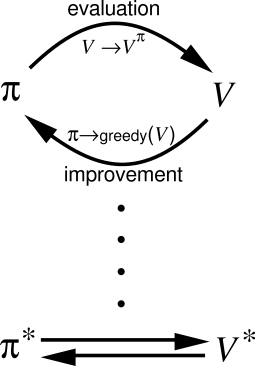
\includegraphics[width=\textwidth]{img/gpi00.png}
	\end{minipage}
	\begin{minipage}[b]{0.55\textwidth}
		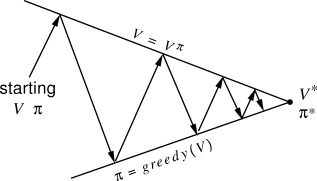
\includegraphics[width=\textwidth]{img/gpi01.png}
	\end{minipage}
	\caption[Generalised Policy Iteration (GPI) schema]{ Generalised policy iteration schema \cite{sutton2018reinforcement}. Value and policy functions compete and cooperate to reach the joint solution: the optimal value function and an optimal policy.}
	\label{fig:gpi}
\end{figure}

\subsection{Model-free approach} \label{mfa}

As reported in the previous section, having a comprehensive knowledge of the environment is at the foundation of dynamic programming methods. However, this fact is not always accurate in practice, where it is infrequent to have a full understanding of how the world works. In these cases, the agent has to infer information using its experience, so it has to exploit model-free methods, based on the assumption that there is no prior knowledge about state transitions and rewards.
This section intends to provide a brief description of two model-free approaches to prediction and control: \textit{Monte Carlo} (MC) methods and \textit{Temporal-Difference} (TD) ones.

\subsubsection{Monte Carlo learning}

Monte Carlo methods \cite[Chapter 6]{sutton2018reinforcement} can learn from episodes of experience using the simple idea that averaging sample returns provide the value. This lead to the main caveat of these methods: they work only with episodic MDPs because the episode has to terminate before it is possible to calculate any returns.
The total reward accumulated in an episode and the distribution of the visited states is used to calculate the value function while the improvement step is carried out by making the policy greedy concerning the value function.

This approach brings to light the exploration dilemma about how it is possible to guarantee that the algorithm will explore all the states without prior knowledge of the whole environment. $\epsilon$-greedy policies are exploited instead of full greedy policy to solve this problem.
An $\epsilon$-greedy policy is a policy that acts randomly with probability $\epsilon$ and follows the policy learned with probability $(1-\epsilon)$.

Unfortunately, even though Monte Carlo methods are simple to implement and they are unbiased because they do not bootstrap, they require a high number of iteration to converge. Furthermore, they have a wide variance in their value function estimation due to lots of random decisions within an episode.

\subsubsection{Temporal Difference learning} \label{tdlearn}

Temporal Difference (TD) is an approach made combining ideas from both Monte Carlo methods and dynamic programming. TD is a model-free method like MC but uses bootstrapping to make updates as in dynamic programming. The central distinction from MC approaches is that TD methods calculate a \textit{temporal error} instead of using the total accumulated reward. The temporal error is the difference between the new estimate of the value function and the old one. Furthermore, they calculate this error considering the reward received at the current time step and use it to update the value function: this means that these approaches can work with continuing (non-terminating) environments.
This type of update reduces the variance compared to Monte Carlo one but increases the bias in the estimate of the value function because of bootstrapping.

The fundamental update equation for the value function is shown in \vref{eq:tdlearning}, where \textit{TD error} and \textit{TD target} are in evidence.
\begin{equation}\label{eq:tdlearning}
	V(s_t) \leftarrow V(s_t) + \alpha \big(\underbrace{\overbrace{r_{t+1} + \gamma V(s_{t+1})}^{\text{TD target}}- V(s_t)}_{\text{TD error} \ (\delta_t)}\big)
\end{equation}
Two TD algorithms for the control problem which are worth quoting because of their extensive use to solve RL problems are \textit{SARSA (State-Action-Reward-State-Action)} and \textit{Q-Learning}.

\textit{SARSA} is an on-policy temporal difference algorithm whose first step is to learn an action-value function instead of a state-value function. This approach leads to focus not to estimate the specific value of each state, but to determine the value of transitions and state-action pairs. \Vref{eq:sarsa} represents the update function of \textit{SARSA}, while \vref{alg:sarsa} summarise its pseudocode.
\begin{equation}\label{eq:sarsa}
	Q(s_t, a_t) \leftarrow Q(s_t, a_t) + \alpha [r_{t+1} + \gamma Q(s_{t+1}, a_{t+1}) - Q(s_t, a_t)]
\end{equation}
\begin{figure}

	\begin{algorithm}[H]
		\SetAlgoLined
		\DontPrintSemicolon
		\LinesNumbered
		\KwIn{step size $\alpha \in (0,1]$, small $\epsilon > 0$\;}
		Initialise $Q(s,a) \; \forall\; s \in \mathcal{S}, a \in \mathcal{A}$ arbitrarily, except that $Q(\text{terminal}, \cdot) = 0$\;
		\ForEach{episode}{
			Initialise $s_t$ \;
			Choose $a_t$ from $s_t$ using policy derived from $Q$ (e.g.\ $\epsilon$-greedy) 	 \;
			\Repeat{$s_t$ is terminal}{
				Take action $a_t$ $\rightarrow$ obtain $r_{t+1}$ and $s_{t+1}$ \;
				Choose $a_{t+1}$ from $s_{t+1}$ using policy derived from Q (e.g.\ $\epsilon$-greedy) \;
				$Q(s_t, a_t) \leftarrow Q(s_t, a_t) + \alpha [r_{t+1} + \gamma Q(s_{t+1}, a_{t+1}) - Q(s_t, a_t)]$\;
				$s_t \leftarrow s_{t+1}$ ; $a_t \leftarrow a_{t+1}$
			}
		}
		\caption{SARSA (on-policy TD control) for estimating $Q \approx q_*$}
		\label{alg:sarsa}
	\end{algorithm}
\end{figure}

\textit{Q-learning} \cite{watkins1989learning} is an off-policy TD control algorithm which represents one of the early revolution and advance in reinforcement learning.
The main difference from SARSA is the update rule for the Q-function: it selects the action in respect of an $\epsilon$-greedy policy while the Q-function is refreshed using a greedy policy based on the current Q-function using a max function to select the best action to do in the current state with the current policy.
\Vref{eq:qlearning} represents the update function of \textit{Q-learning}, while \vref{alg:qlearning} summarise its pseudocode.
\begin{equation}\label{eq:qlearning}
	Q(s_t, a_t) \leftarrow Q(s_t, a_t) + \alpha [r_{t+1} + \gamma \max_{a}{Q(s_{t+1}, a)} - Q(s_t, a_t)]
\end{equation}
\begin{figure}

	\begin{algorithm}[H]
		\SetAlgoLined
		\DontPrintSemicolon
		\LinesNumbered
		\KwIn{step size $\alpha \in (0,1]$, small $\epsilon > 0$\;}
		Initialise $Q(s,a) \; \forall\; s \in \mathcal{S}, a \in \mathcal{A}$ arbitrarily, except that $Q(\text{terminal}, \cdot) = 0$\;
		\ForEach{episode}{
			Initialise $s_t$ \;
			Choose $a_t$ from $s_t$ using policy derived from $Q$ (e.g.\ $\epsilon$-greedy) 	 \;
			\Repeat{$s_t$ is terminal}{
				Take action $a_t$ $\rightarrow$ obtain $r_{t+1}$ and $s_{t+1}$ \;
				Choose $a_{t+1}$ from $s_{t+1}$ using policy derived from Q (e.g.\ $\epsilon$-greedy) \;
				$Q(s_t, a_t) \leftarrow Q(s_t, a_t) + \alpha [r_{t+1} + \gamma \max_{a}{Q(s_{t+1}, a)} - Q(s_t, a_t)]$\;
				$s_t \leftarrow s_{t+1}$ ; $a_t \leftarrow a_{t+1}$
			}
		}
		\caption{Q-learning (off-policy TD control) for estimating $\pi \approx \pi_*$}
		\label{alg:qlearning}
	\end{algorithm}
\end{figure}

\subsubsection{Temporal Difference Lambda Learning}

As reported previously, Monte Carlo and Temporal Difference learning perform updates in different ways. The first approach exploits the total reward to update the value function, while the second one, on the other hand, works with the reward of the current step. Temporal Difference Lambda, also known as TD($\lambda$) \cite[Chapter 7,12]{sutton2018reinforcement}, represents a combination of these two procedures and it takes into account the results of each time step together with the weighted average of those returns.
The idea of calculating TD target looking n-steps into the future instead of considering only a single step is the baseline of TD($\lambda$). This lead to the formalisation of the $\lambda$-weighted return $G_t^\lambda$ presented in \vref{eq:lambdaG}.
\begin{equation}\label{eq:lambdaG}
	G_t^\lambda = (1-\lambda)\sum_{n=1}^{\infty}\lambda^{n-1}G_t^{(n)}
\end{equation}
TD($\lambda$) implementation takes into account an additional variable called eligibility trace $e_t(s_t)$ which indicates how much learning should be carried out for each state for each timestep. It aims to describe how much the agent encountered a specific state recently and \vref{eq:eligibility_trace} describes the updating rule of this value where the $\lambda$ represents the trace-decay parameter.
\begin{equation}\label{eq:eligibility_trace}
	e_t(s) = \gamma \lambda e_{t-1}(s) + \mathbbm{1}(s = s_t)
\end{equation}

\subsection{Model-based approach}


Heretofore, the focus of this section was on methods which have no prior knowledge of the environment, since this thesis grows on model-free foundations.
Despite this point, it is worth to summarise the main concepts behind model-based approaches.
Model-based methods gather information to enable the ability of planning, which can enhance the sample efficiency of the algorithm.

There are two primary principles to model-based learning. The first one implies to assemble a model starting from prior knowledge and to exploit it to calculate the policy and the value-function, while the second one is to infer the model from the environment by sampling experience.
The central drawback of the first technique is that prior knowledge could be not as accurate as expected, leading to sub-optimal results. Consequently, the preferred way to learn is the second one.

The decisive point behind these approaches is that they are more sample-efficient concerning model-free ones: they require fewer data to learn a policy. On the other hand, the algorithm must learn the policy as well as the model: this translates to two different sources of approximation errors and an increase of computational complexity.

\section{Deep reinforcement learning} \label{deepreinflearn}

%\todomacaluso{
%	\begin{itemize}
%		\item Introduction and motivation behind function approximation
%		\item Value-based methods and Policy Gradient methods
%		\item Focus and detailed description of DDPG and SAC
%	\end{itemize}	
%}


The strategies shown so far works smoothly with systems with well-defined states and actions. In this context, it is reasonable to use lookup tables to describe the problem: state-value function V has an entry for each state while action-value function Q has an entry for each state-action pair.
It is easy to understand how this setting cannot scale up with very large MDPs: problems regarding the availability of memory arise as it becomes difficult to manage the storage of a large number of states and actions. Also, there may be obstacles concerning the slowness of learning the value of each state individually. Furthermore, the tabular form could lead to expensive computation in linear lookup and can not work with continuous action and state spaces.

Function approximators represent the solution to overwhelm this problem. The underlying intention is to use a vector $\theta = (\theta_1, \theta_2. \dots, \theta_n)^T$ to estimate state-value and action-value function as shown in \vref{eq:fun_appr}, generalise from seen states to unseen states and finally update parameter $\theta$ using MC or TD Learning strategies.
\begin{equation}\label{eq:fun_appr}
	\begin{aligned}
		V(s, \theta)    & \approx V_\pi(s)   \\
		Q(s, a, \theta) & \approx Q_\pi(s,a)
	\end{aligned}
\end{equation}
In these terms, function approximators can be considered as a mapping from the vector $\theta$ to the value function.
This choice leads to a reduction in the number of parameters to learn and consequently to a system which can generalise better in fewer training samples.

Nowadays, since its widespread use in research, neural networks represent the most intuitive option to take as function approximator: it reduces the training time for high dimensional systems, and it requires less space in memory.
This point represents the bridge between traditional reinforcement learning and recent discoveries in the theory of deep learning.
Thanks to the last decade great fervour of deep learning, neural networks have become the fundamental tool to exploit as function approximator to develop deep reinforcement learning (Deep RL) which accomplished remarkable results. One of the first steps towards Deep RL and general artificial intelligence -- an AI broadly applicable to a different set of various environments -- was done by DeepMind with their pioneering paper \cite{mnih2013playing} and the consequent \cite{mnih2015human}.

Because of the nature of this work, the focus of this section will be on model-free algorithms.
This section aims to explain the state-of-the-art and the leading theory behind Deep RL framework together with an overview about deep learning and the presentation of two deep actor-critic algorithms used in the experiments of this thesis: Deep Deterministic Policy Gradient (DDPG) and Soft Actor-Critic (SAC).

\subsection{Fundamentals of Deep Learning}

\subsubsection{Artificial Neural Networks}
Deep learning (DL) is an approach to learning based on a function $f: \mathcal{X} \rightarrow \mathcal{Y}$ parametrised with $w \in \mathbb{R}^{n_w} (n_w \in \mathbb{N})$ such that $y = f(x;w)$.

The starting point of this research field is the artificial neuron, inspired by the biological neuron from the brain of animals and human being. A neuron consists of numerous inputs called \textit{dendrites} coming from preceding neurons. Therefore, the neuron elaborates the input and, only if the value reaches a specific potential, it \textit{fires} through its single output called \textit{axon}.

The neuron elaborates the inputs by taking the weighted sum, adding a bias $b$ and applying an activation function $f$ following the relation $y = f( \sum_{n}w x_i + b)$. \Vref{fig:neuron} shows the parallel comparison between the biological neuron and the artificial one. The set of parameter $w$ needs to be adjusted to find a good parameter set: this process is called \textit{learning}.
\begin{figure}[!h]
	\centering
	\begin{minipage}[b]{0.47\textwidth}
		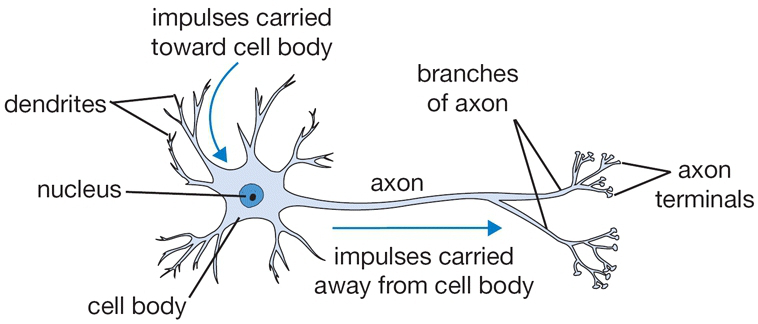
\includegraphics[width=\textwidth]{img/neuron.png}
		\vspace{2mm}
	\end{minipage}
	\begin{minipage}[b]{0.5\textwidth}
		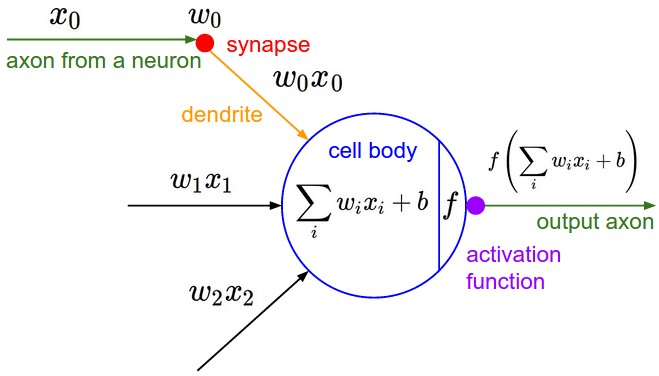
\includegraphics[width=\textwidth]{img/neuron_model.jpeg}
	\end{minipage}
	\caption[Comparison between Biological and Artificial Neuron]{Comparison between biological neuron (left) and artificial neuron (right). The artificial neuron designs the dendrites as weighted inputs and returns the sum through an activation function. \cite{stanford2019cs231n}.}
	\label{fig:neuron}
\end{figure}

A deep neural network (NN) organises a set of artificial neurons in a series of processing layers to which correspond non-linear transformation.
The whole sequence of these alterations directs the learning process through different levels of abstraction \cite{erhan2009visualizing}.
To better understand the nature of a deep neural network, it is convenient to describe a neural network with one fully-connected layer represented by \vref{fig:fullyconnected}.
\begin{equation}\label{eq:non_linear_transformation}
	\begin{gathered}
		h = g(w_1 \cdot i + b_1) \\
		o = w_2 \cdot h + b_2
	\end{gathered}
\end{equation}
\begin{figure}
	\centering
	\tikzset{%
		every neuron/.style={
				circle,
				draw,
				minimum size=1cm
			},
		neuron missing/.style={
				draw=none,
				scale=4,
				text height=0.333cm,
				execute at begin node=\color{black}$\vdots$
			},
	}
	\resizebox{0.6\textwidth}{!}{
		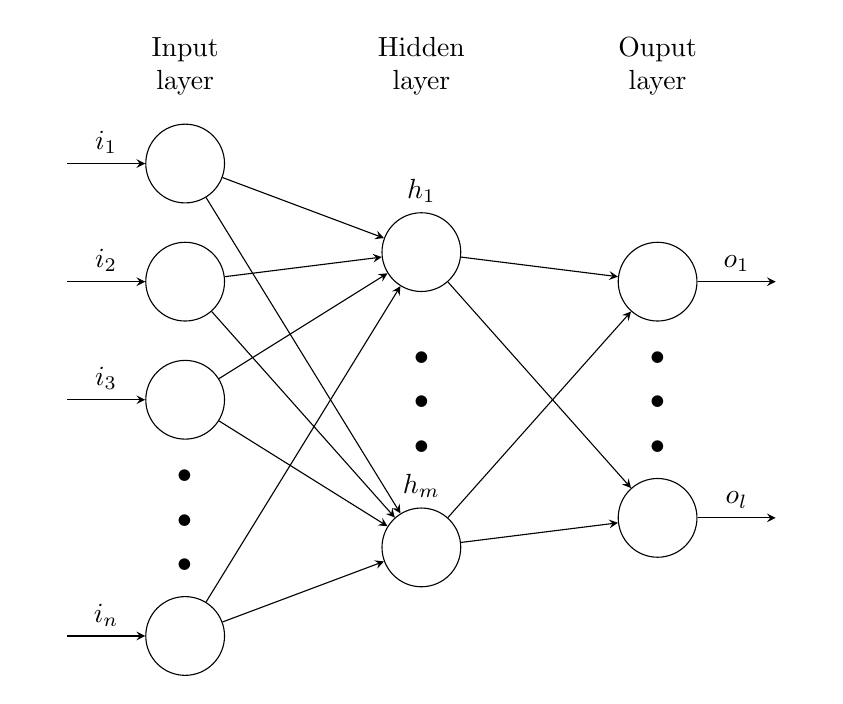
\begin{tikzpicture}[x=1.5cm, y=1.5cm, >=stealth]

			\foreach \m/\l [count=\y] in {1,2,3,missing,4}
			\node [every neuron/.try, neuron \m/.try] (input-\m) at (0,2.5-\y) {};

			\foreach \m [count=\y] in {1,missing,2}
			\node [every neuron/.try, neuron \m/.try ] (hidden-\m) at (2,2-\y*1.25) {};

			\foreach \m [count=\y] in {1,missing,2}
			\node [every neuron/.try, neuron \m/.try ] (output-\m) at (4,1.5-\y) {};

			\foreach \l [count=\i] in {1,2,3,n}
			\draw [<-] (input-\i) -- ++(-1,0)
			node [above, midway] {$i_\l$};

			\foreach \l [count=\i] in {1,m}
			\node [above] at (hidden-\i.north) {$h_\l$};

			\foreach \l [count=\i] in {1,l}
			\draw [->] (output-\i) -- ++(1,0)
			node [above, midway] {$o_\l$};

			\foreach \i in {1,...,4}
			\foreach \j in {1,...,2}
			\draw [->] (input-\i) -- (hidden-\j);

			\foreach \i in {1,...,2}
			\foreach \j in {1,...,2}
			\draw [->] (hidden-\i) -- (output-\j);

			\foreach \l [count=\x from 0] in {Input, Hidden, Ouput}
			\node [align=center, above] at (\x*2,2) {\l \\ layer};

		\end{tikzpicture}
	}
	\caption[Fully-connected layer representation]{An example representation of a deep neural network with one fully-connected hidden layer.}
	\label{fig:fullyconnected}
\end{figure}
The input layer receives as input a column vector of input-features $i$ of size $n \in \mathbb{N}$. Every value of the hidden-layer represented by a vector $h$ of size $m \in \mathbb{N}$ is the result of a transformation of the input values given by \vref{eq:non_linear_transformation} where $w_1$ is a matrix of size $m \times n$ and $b_1$ is a bias term of size $m$. $g$ is a non-linear parametric function called activation function, which represents the core of neural networks. Subsequently, the second and last transformation manipulates the hidden layer $h$ to produce the values of the output layer following \vref{eq:non_linear_transformation} using $w_2$ with size $o \times m$ and $b_2$ with size $o$.

\subsubsection{Learning process}

The learning process aims to seek a set of parameters $\theta$ that results in the best possible function approximation for a specific objective. In supervised learning, the actual output $Y$ is available for each particular input $X$, and it is used to update the parameters. The learning process can be carried out iteratively according to the following steps.

\paragraph{Forward pass} The input $X$ is forwarded through the neural network and the output $Y_{pred} = f(X, \theta)$ is gathered.

\paragraph{Loss} The resulting predicted value $Y_{pred}$ is compared with the actual value $Y$ computing the loss function $L(\theta)$. There are a lot of loss functions available to satisfy the particular needs of specific learning tasks. The \textit{error} is the difference between the output of the neural network for a specific input data and the actual value: it is essential to calculate the loss function. One of the most exploited loss function is the \textit{Mean-Squared Error} (MSE) \cite{shalev2014understanding} shown in \vref{eq:backprop} which works with L2-distance.

\begin{equation}\label{eq:backprop}
	\begin{aligned}
		L(y, \hat{y}) = (y_\theta - y)^2 \\
		J = \frac{1}{n}\sum_{i=1}^{n}L(y_i, f(x_i))
	\end{aligned}
\end{equation}

\paragraph{Backpropagation}
The next step is the computation of the global gradient of the loss function $\nabla L(\theta)$, which is carried out together with its backpropagation through the network. The backpropagation algorithm \cite{rumelhart1988learning} calculates the local gradient of loss for each neuron in the hidden layers. The concept underlying this procedure and shown in \vref{eq:chainrule} is the \textit{chain rule} \cite{lecun2015deep}, which computes derivatives of composed functions by multiplying local derivatives.
\begin{equation}\label{eq:chainrule}
	\begin{gathered}
		y = g(x), \;\;\; z = f(g(x)),  \;\;\;
		\frac{\partial z}{\partial x} = \frac{\partial z}{\partial y} \frac{\partial y}{\partial x}
	\end{gathered}
\end{equation}
Therefore, the chain rule is exploited to propagate the calculated global gradient loss $\frac{\partial L(\theta)}{\partial \theta}$ back through the network, in the opposite direction of the forward pass.
The procedure calculates the local derivatives during the forward pass, while estimates the local gradient of loss during backpropagation determining the multiplication between the local derivative and the local gradient of the loss of the connected neuron of the next layer: if the neuron has multiple connections neurons, the algorithms adds up all the gradients.

\paragraph{Update} The final step consists in the update of the weights of all neurons. There are many ways developed through the years to carry out the update phase, but the most common one is the gradient descent.
The objective of the gradient descent is to minimise the loss function by refreshing the internal parameters of the network in the negative direction of the gradient loss: this choice leads the function approximation process closer to the minimum at each iteration. \Vref{eq:update} describes the update rule presented by the gradient descent where $\alpha$ is the learning rate. The last-mentioned parameter determines how quickly the algorithm should approach the minimum. A higher learning rate leads to a more significant step towards the minimum, which threatens to overshoot the target.
\begin{equation}\label{eq:update}
	\theta \leftarrow \theta -\alpha \nabla_\theta J
\end{equation}
Nowadays, the technique applied in the majority of research projects is stochastic gradient descent (SGD) which combines batch learning \cite{stanford2019cs231n} and gradient descent, but also its various improved extensions and variants, such as ADAM \cite{kingma2014adam} and AdaGrad \cite{duchi2011adaptive}: these extensions manage to improve the convergence of SGD thanks to the introduction of adaptive learning rates.

\subsubsection{Regularisation}

The final aim of the learning process is to obtain a function approximator capable of generalising over data. This fact means that a neural network should show performances on unseen data comparable to the one obtained from training data. For this reason, it is necessary an appropriate trade-off between underfitting and overfitting.

A shallow approximated function and insufficient training data with a lack of diversity are the leading cause to the first situation: the network generalises on the data, but the prediction error is always too high for all data points.
The phenomenon of overfitting describes the exact contrary of underfitting. The leading cause is a too complex approximation function: this lead to a network which scores an excellent performance on training data, but poorly predicts unseen points.

Regularisation \cite{bishop2006pattern,lecun2015deep} represents an approach to overcome and prevent the problem of overfitting. It works extending the loss function with a regularised term $\Omega(\theta)$ as shown in \vref{eq:generalreg} where $\lambda$ is the regularisation factor.
\begin{equation}\label{eq:generalreg}
	L'(\theta) = L(\theta, Y, Y_{pred}) + \lambda \Omega(\theta)
\end{equation}
\Vref{eq:l2reg,eq:l1reg} show two examples of regularisation terms. The first is $L^2$-regularisation which exploits the squared sum of the weights $\theta$ in order to keep the weights small. The second approach is known as $L^1$-regularisation: in this case, large weights are less penalised, but this method leads to a sparser solution.
\begin{equation}\label{eq:l2reg}
	L'(\theta) = L(\theta, Y, Y_{pred}) + \lambda \frac{1}{2}||\theta||^2
\end{equation}
\begin{equation}\label{eq:l1reg}
	L'(\theta) = L(\theta, Y, Y_{pred}) + \lambda \frac{1}{2}||\theta||
\end{equation}


\subsubsection{Activation function}

\Vref{eq:activation} shows the most common activation functions: in general, \textit{ReLu}  achieves better performance over a wide variety of tasks, but usually the selection of the best activation function has to be done starting from all information and requirements of the deep learning model.
\begin{equation}\label{eq:activation}
	\begin{aligned}
		\text{Sigmoid} \;\rightarrow\;                      & g(x) = \frac{1}{1+ e^{-x}}           \\
		\text{Hyperbolic Tangent} \;\rightarrow\;           & g(x) = \frac{e^x-e^{-x}}{e^x+e^{-x}} \\
		\text{Rectified Linear Unit (ReLu)} \;\rightarrow\; & g(x) = \max(0,x)
	\end{aligned}
\end{equation}

\subsubsection{Batch Learning and Normalisation}
The basic concept underlying \textit{batch learning} \cite{stanford2019cs231n} is to process a set of $n$ training samples called also \textit{mini-batches} in the place of a single one. This method works with the gradient averaged over all the samples in the mini-batch: it leads to a more accurate gradient reducing its variance and the training time.

\textit{Batch normalisation} consists of zero-centring and rescaling all data in a specific batch, resulting in a  mean of normalised data close to $0$ and a variance close to $1$. The algorithm presented in \vref{alg:batchnorm} is the one provided in \cite{ioffe2015batch}.
This method computes the mean $\mu_\beta$ and the variance $\sigma_\beta$  element-wise for each spatial position in the batch: $\epsilon > 0$ is a small value to avoid the division by zero.
The batch normalisation layer then processes the resulting normalised value: $\gamma$ and $\beta$ are the parameters of this layer that are in addition to the original parameter set $\theta$ of the neural network in the learning process.
The new learning dynamic provided by the addition of this class of layer increases the network expressivity: applying this method to the input data and the output of any hidden layer results in the reduction of the training time, better regularisation during learning and the reduction of the overfitting phenomenon.
\begin{figure}
	\begin{algorithm}[H]
		\SetAlgoLined
		\setstretch{1.35}
		\DontPrintSemicolon
		\LinesNumbered
		\KwIn{Mini-batch $\mathcal{B} = {x_{1 \dots m}}$; $\gamma$ and $\beta$ prameters to be learned\;}
		\KwOut{$y_i = \text{BN}_{\gamma, \beta}(x_i)$}
		$\mu_\beta \leftarrow \frac{1}{m} \sum_{i=1}^{m} x_i $ \tcp*{Mini-batch mean}
		$\sigma_\beta^2 \leftarrow \frac{1}{m} \sum_{i=1}^{m} (x_i-\mu_\beta)^2 $ \tcp*{Mini-batch variance}
		$\hat{x_i} \leftarrow \frac{x_i - \mu_\beta}{\sqrt{\sigma^2_\beta + \epsilon}} $\tcp*{Normalisation}
		$y_i \leftarrow \gamma \hat{x_i} + \beta \equiv \text{BN}_{\gamma, \beta}(x_i)$\tcp*{Scale and shift}
		\caption{Batch normalisation}
		\label{alg:batchnorm}
	\end{algorithm}
\end{figure}

\subsubsection{Convolutional Neural Networks}

Sensory reception represents how humans and animals react to changes: it consists of sensors which process the input data and are sensitive to specific stimuli.
This system inspired the architecture underlying Convolutional Neural Networks: they could efficiently handle significant input data with many applications in computer vision.
\Vref{fig:lenet5} displays the \textit{LeNet-5} \cite{lecun1998gradient} which is capable to recognise digits in images. It represents a perfect example of a standard convolutional neural network architecture: it consists of a series of convolutional layers followed by a subsampling pooling layer.
At the end of the convolutional stack, the values map into final hidden layers of the network to compute the final low-dimensional output of the network: fully-connected layers usually compose these final layers.
It is possible to suppose that the first layers have to learn low-level features of the input data while succeeding layers are responsible for combining the last-mentioned features in high-level ones.

\begin{figure}[!h]
	\centering
	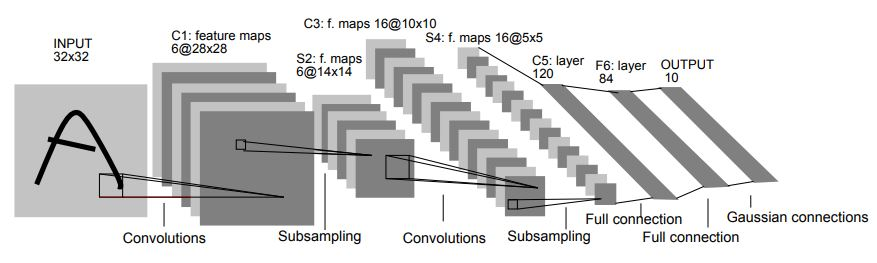
\includegraphics[width=\textwidth]{img/lenet5.jpg}

	\caption{ Comparison between biological neuron (left) and artificial neuron (right). The artificial neuron designs the dendrites as weighted inputs and returns the sum through an activation function. \cite{stanford2019cs231n}.}
	\label{fig:lenet5}
\end{figure}

\paragraph{Convolutional Layer}

Convolutional layers \cite{lecun1995convolutional} operates with a set of learnable filters (called kernels) with dimensions $n \times m$ smaller than the whole input image. The convolution is the basic operation employed in these class of layer: it consists in convolving each filter across the width and height of the input data and computing dot products between the values in the filter and the ones in the input at any position. The result of this operation is a 2-dimensional activation map that contains the results of that filter at every spatial position.  In this context, the network can learn filters that detect specific features in the image such as edges, textures and patterns \cite{erhan2009visualizing}.

It is possible to compute the output size $W_2 \times H_2 \times D_2$ of a convolutional layer starting from the input size $W_1 \times H_1 \times D_1$ and from the hyperparameters of this class of layer: the number of filters $K$, their spatial extent $F$, the stride $S$ and the amount of zero padding $P$. The resulting volume size can be calculated using the relations reported in \vref{eq:conv}.
\begin{equation} \label{eq:conv}
	\begin{aligned}
		W_2 & = (W_1 - F + 2P)/S + 1 \\
		H_2 & = (H_1 - F + 2P)/S + 1 \\
		D_2 & = K
	\end{aligned}
\end{equation}
The number of parameters introduced by a single kernel is equal to $F \cdot F \cdot D_1$, so the convolutional layer has a total of $(F \cdot F \cdot D_1) \cdot K$ weights and $K$ bias.

In a convolutional layer, the number of weights is kept small and then the computation is more efficient than the one of a fully-connected layer: small filters need fewer parameters and less work in the convolutional operation. Besides this motivation, the filters are kept small also because it makes them capable of learning small and low-level features. The great innovation behind convolutional layers is that the same neuron can recognise the related learned features even if they emerge in different locations of the image: this is the property of translation invariance of feature detection.

\paragraph{Pooling Layer}

It is common to insert a pooling layer in-between successive convolutional layers. The main objective of this class of layers is to apply a downsampling filter on the input: it progressively reduces the spatial size of the representation, decreasing the number of parameters and the computational cost in the network. It is also useful to control overfitting.

It is possible to compute the size of the output $W_2 \times H_2 \times D_2$ of a pooling layer using starting from the size of the input $W_1 \times H_1 \times D_1$ and from the hyperparameters of this class of layer: the spatial extent of the filter $F$, the stride $S$. The resulting volume size can be calculated using the relations reported in \vref{eq:pool}.
\begin{equation} \label{eq:pool}
	\begin{aligned}
		W_2 & = (W_1 - F)/S + 1  \\
		H_2 & = (H_1 - F )/S + 1 \\
		D_2 & = D_1
	\end{aligned}
\end{equation}
The most common types of pooling layer are the \textit{max-pooling} and the \textit{average-pooling} layer. Both classes return a single value for each position of the filter: the first returns the maximum value, while the second returns the average among the values in the specific section of the input.



\begin{figure}[!h]
	\centering
	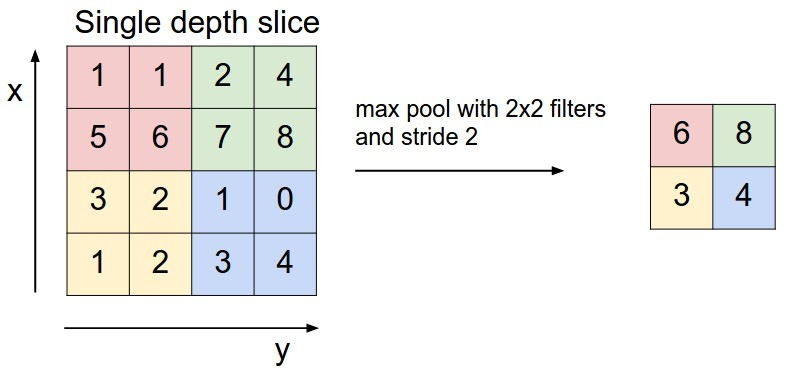
\includegraphics[width=0.7\textwidth]{img/maxpool.jpeg}
	\caption[Max-Pooling layer example]{Example of a max-pooling operation with a stride of 2 and a spatial extent of 2. \cite{stanford2019cs231n}.}
	\label{fig:avgpool}
\end{figure}

It is worthy of using a pooling layer in a situation where the exact feature position is not relevant but rather whether a particular feature exists in the input at all.
Increasing the stride of convolutional layers represent an alternative approach to downsample without the usage of max-pooling layers \cite{springenberg2014striving}.


\subsection{Value-based methods}

The first class of algorithms to explore is value-based one. They works learning an approximator $Q_\theta(s,a)$ to infer the optimal action-value function $Q^*(s,a)$ using an objective function based on Bellman equations.
The preponderance of optimisations belonging to this category is \textit{off-policy}: this means that the optimisation step is done using all data collected during the whole training, not only with the most recent policy available. In this configuration, the information used for the learning phase could also come from exploration decision, apart from ones obtained with the most recent policy.
Indeed, value-based approaches are more sample efficient because they can reuse data more efficiently, but they are considered less stable than policy gradient ones.
Thanks to the relation expressed by $a(s) = \operatornamewithlimits{argmax}_a Q_\theta(s,a)$, it is possible to obtain the policy learned so far from the current action-value function.

\subsubsection{Deep Q-Network (DQN)}
This algorithm grows from the ideas underlying Q-Learning \cite{watkins1989learning}  shown previously in \vref{tdlearn}. The team of DeepMind introduced the Deep Q-Network (DQN) in \cite{mnih2013playing} and in the next cutting-edge paper \cite{mnih2015human}: they managed to create an algorithm capable of learning to play ATARI video-games online using raw image and pixels. It works with neural networks as a function approximator, employing convolutional layers as first layers of the neural network and performing the optimisation with a variant of stochastic gradient descent called RMSprop \cite{tieleman2012lecture}. The exploited neural network provides as output a probability distribution over all possible discrete actions to determine what is the best action to take.

To overcome the instability problem of value-based methods, DQN utilises two heuristics to narrow instabilities.

\paragraph{Target Network}
The presence of a second network, also called  \textit{target network}, enriches the update phase of this algorithm. \Vref{eq:lossdqn}
defines the loss function of DQN where $y_i$ value is computed using the target network instead of the local network. Therefore, the parameters of the target network are hard updated every $I \in \mathbb{N}$ iterations: this choice precludes instabilities and avoids divergence because of target networks parameters remain fixed for $I$ iterations.
\begin{equation} \label{eq:lossdqn}
	\begin{gathered}
		L_i(\theta_i) = \mathbb{E}_{s, a \sim \pi}\big[(y_i - Q(s, a; \theta_i))^2\big]\\
		y_i = \mathbb{E}_{s' \sim E}[r + \gamma \max_{a'}Q(s',a'; \theta_{i-1})|s,a]
	\end{gathered}
\end{equation}

\paragraph{Experience Memory Replay} \label{experience}

Another crucial introduction in this algorithm is \textit{experience memory replay buffer} \cite{lin1992self}. Trajectories sampled from the environment are temporally correlated, and this could lead to overfitting the parameters of the neural network because the data are not independent and identically distributed (\textit{i.i.d.}). The setting of this algorithm is \textit{online} because the replay buffer stores $N_{\text{replay}} \in \mathbb{N}$ replacing old steps as new ones arrive. The experience is collected as tuples $(s_t,a_t,r_t,s_{t+1})$ using the $\epsilon$-greedy policy. The learning phase samples a set of limited tuples called \textit{mini-batch} allowing a wider set of state-action pair in the update of the network and improving the procedure in terms of variance in respect of single tuple update.
Trajectories sampled from the environment are temporally correlated, and this could lead to overfitting the parameters of the neural network. Using a batch sample from the replay buffer makes the data \textit{i.i.d.} and consequently improves the learning.

\subsubsection{Improvements of DQN}
Further investigation and speculation followed the publication of the thriving DQN. Summing up and comparing these new approaches to original DQN is the main aim of \textit{Rainbow} \cite{hessel2018rainbow}: it also introduces an algorithm called \textit{Rainbow DQN} with all the techniques proposed. The following paragraphs will delineate three main improvements of DQN.

\paragraph{Double DQN}
The double DQN \cite{hasselt2010double, van2016deep} improvement can handle the intricacy of overestimation of Q-values caused by the maximisation step in \vref{eq:lossdqn}. It works with two separate Q-Network with parameters $\theta$ and $\theta^-$ for estimating TD-target. It allows for removing the positive bias in estimating action values, leading to less overestimation of Q-learning values, improved stability and performance. In this context, the target $y_i$ is replaced by \vref{eq:ddqny}.
\begin{equation} \label{eq:ddqny}
	y_i = \mathbb{E}_{s' \sim E}[r + \gamma Q(s',\operatornamewithlimits{argmax}_aQ(s', a; \theta_{i-1}); \theta^-_{i-1})|s,a]
\end{equation}
\paragraph{Prioritised Experience Replay}

The fundamental idea underlying \textit{prioritised experience replay} \cite{schaul2015prioritized} is precisely to prioritise experiences that contain more crucial information than other ones. An additional value that defines the priority of a specific transition joins each tuple stored in the replay buffer: thanks to this approach, experiences with higher priority has a higher sampling probability and are more likely to remain longer in the replay buffer. It is possible to use \textit{TD-error} to measure the importance of each tuple in the experience. A high TD-error means that the agent behaved better or worse than expected in that particular moment, and therefore, it can learn more from that specific passage.

\paragraph{Dueling DQN}

The dueling DQN architecture \cite{wang2015dueling} presented in \vref{fig:duelingdqn} works decoupling the Q-value estimation in two distinct sequences of fully-connected layers right after convolutional layers.
\begin{figure}
	\centering
	\resizebox{0.6\textwidth}{!}{
		\begin{tikzpicture}
			\node at (0,0) (image) {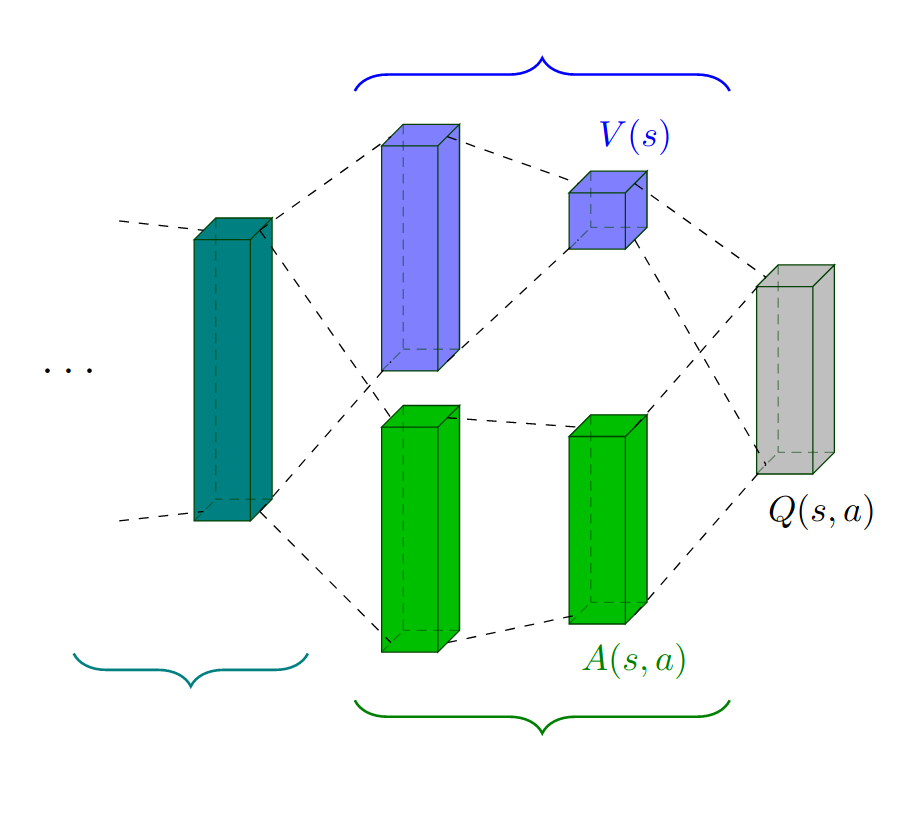
\includegraphics[width=0.7\textwidth]{img/duelingdqnn.png}};
			% node a_t
			\node[mylabel, below right=-0.1cm and -0.5cm of image.north] (action) {\LARGE \textcolor{Blue}{$\beta$}};
			\node[mylabel, above right=0.3cm and -0.5cm of image.south] (action) {\LARGE \textcolor{OliveGreen}{$\alpha$}};
			\node[mylabel, above right=0.8cm and -4.6cm of image.south] (action) {\LARGE \textcolor{PineGreen}{$\theta$}};% node s_t
		\end{tikzpicture}
	}
	\caption[Dueling DQN]{ Dueling DQN architecture \cite{wang2015dueling}: It consists in two stream to estimate state-value parametrised with $\beta$ and advantages values parametrised with $\alpha$ for each action. The last layer represent the combination of these two types of values to obtain the Q-function. \cite{franccois2018introduction}}
	\label{fig:duelingdqn}
\end{figure}

These streams are capable of providing separate estimates of the state-value  $V(s; \theta, \beta)$ and advantage $A(s,a; \theta, \alpha)$ functions exploited in the end to obtain the Q-value function $Q(s,a; \theta, \alpha, \beta)$ estimate where $\theta$ represents the parameters of convolutional layers while $\alpha$ and $\beta$ the ones of state-value and advantage function respectively.

The first formalisation of the Q-value function is shown by \vref{eq:qvalueddqn0}, but \cite{wang2015dueling} also suggests a different approach shown in \vref{eq:qvalueddqn1} with increased stability in practice.
\begin{gather}
	Q(s,a; \theta, \alpha, \beta) = V(s;\theta, \beta) + \big(A(s,a;\theta, \alpha) - \max_{a' \in \mathcal{A}}A(s, a'; \theta, \alpha)\big) \label{eq:qvalueddqn0}\\
	Q(s,a; \theta, \alpha, \beta) = V(s;\theta, \beta) + \big(A(s,a;\theta, \alpha) - \frac{1}{|\mathcal{A}|}\sum_{a' \in \mathcal{A}}A(s, a'; \theta, \alpha)\big) \label{eq:qvalueddqn1}
\end{gather}



\subsection{Policy gradient methods}

Policy gradient algorithms aim to optimise the policy performance measure in \vref{eq:pgperf} by finding a suitable policy $\pi_\theta(s|a)$ capable of generating a trajectory $\tau$ that maximises the expected rewards \vref{eq:pgmax} instead of learning a  value function. Indeed the objective function in policy gradient methods consists of maximising $J(\theta)$ value by finding a proper policy by updating $\theta$ parameters directly.
\begin{gather}
	J(\theta) = \mathbb{E}\Bigg[\sum_{t=0}^{N}r(s_t,a_t); \pi_\theta\Bigg] = \sum_{\tau}P(\tau;\theta)r(\tau) \label{eq:pgperf}\\
	\theta^* = \operatornamewithlimits{argmax}_\theta J(\theta) \label{eq:pgmax}
\end{gather}
Stochastic gradient ascent is used to refresh the parameters of the policy $\theta$. Gradient ascent is the inverse of gradient descent and updates the parameters $\theta_t$ in the positive direction of the gradient of the policy’s performance measure $\nabla_\theta J(\theta)$ following \vref{eq:pgascent} where $\alpha$ is the learning rate which defines the strength of the steps in the direction of the gradient.
\begin{equation}
	\theta_{t+1} \leftarrow \theta_t + \alpha \nabla_\theta J(\theta_t) \label{eq:pgascent}
\end{equation}
The main advantage of policy gradient approaches consists in the stability of their convergence: these methods work updating their policy directly at each time step instead of renewing value function from which to derive the policy like value-based methods. Last-mentioned approaches can lead to a radical change in the policy output even for a small change in the value function: this event can cause prominent oscillation during training.
Furthermore, policy gradient algorithms can face infinite and continuous action space because the agent estimates the action directly instead of calculating the Q-value for each possible discrete action.
The third feature is their ability to learn stochastic policies, useful in uncertain contexts or partially observable environments.
Despite the presence of the advantages just mentioned, policy gradient methods have an substantial disadvantage: they tend to converge to a local maximum instead of the global optimum.

\subsubsection{Actor-Critic Architecture}

Actor-critic architecture, shown in \vref{fig:actorcritic}, represents the point of contact between value-based approaches and policy gradient methods. They are policy gradient methods basically but exploit value-function to learn the parameters $\theta$ of the policy. As its name suggests, these approaches work with two different parts called \textit{actor} and \textit{critic} \cite{konda2000actor}. The \textit{actor} relates to the policy, while the \textit{critic} deals with the estimation of a value function (e.g.\ Q-value function). In the context of deep reinforcement learning, they can be represented using neural networks function approximator \cite{mnih2016asynchronous}: the actor exploits gradients derived from the policy gradient theorem and adjusts the policy parameters, while the critic estimates the approximate value function for the current policy $\pi$.

Standard practice is to update both networks with the \textit{TD-Error}, discussed in \vref{tdlearn}. Estimation made by the critic is useful to determine the contribution that expected values of the current and next state gives to the TD-error. Essentially, the output of the critic contributes to the update of the actor.


\begin{figure}[!h]
	\centering
	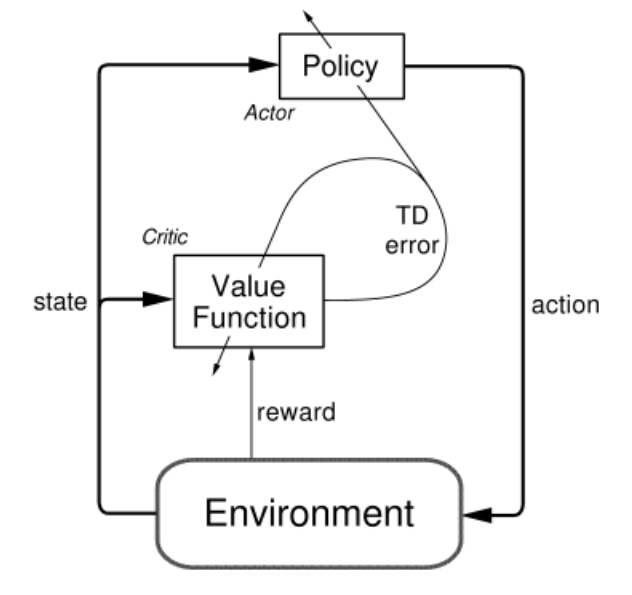
\includegraphics[height=0.4\textwidth]{img/actorcritic.png}
	\caption[Actor-Critic architecture schema]{Actor-critic architecture schema: the actor represents the policy and maps the input state to an output action, while the critic represents the value function. Both networks can be updated using the contribution of the critic. It is noticeable that the actor uses the critic during the learning process \cite{sutton2018reinforcement}.}
	\label{fig:actorcritic}
\end{figure}

\subsection{Deep Deterministic Policy Gradient (DDPG)} \label{ddpg}

Deep Deterministic Policy Gradient (DDPG) \cite{lillicrap2015continuous} is a policy gradient algorithm that works learning a Q-function and a policy, and that grows from the deterministic policy gradient algorithm (DPG) \cite{silver2014deterministic}. It is a model-free, off-policy, actor-critic algorithm which utilises deep function approximators to learn policies in high-dimensional, continuous action spaces. It can be applied to situations that can not be solved using \textit{DQN} algorithm \cite{mnih2015human} because of the presence of continuous action spaces. A fine discretisation of the action space to adapt the situation to DQN would lead to an explosion in the number of discrete actions and the curse of dimensionality.
\textit{Bellman equation} and \textit{Q-learning} are integral parts of this algorithm. The algorithm concurrently learns a Q-value function and a policy: it uses off-policy data and the Bellman equation to learn the Q-value function and uses the Q-value function to learn the policy.

Usually, in reinforcement learning, if the optimal action-value function $Q^*(s,a)$ is known, then in any given state, the optimal action $a^*(s)$ can be found by solving \vref{eq:besta}.
\begin{equation} \label{eq:besta}
	a^*(s) = \arg \max_a Q^*(s,a)
\end{equation}
When the number of discrete actions is finite, calculating the $\max$ poses no problem, because the Q-values can be calculated for each action separately, then directly compared. However, when the action space is continuous, this process becomes highly non-trivial: it would need to be run at every step of the episode, whenever the agent wants to take any action in the environment, and this can not work.

Because the action space is continuous, the function $Q^*(s,a)$ is presumed to be differentiable concerning the action argument. For this reason, an efficient, gradient-based learning rule for a policy $\pi(s)$ which exploits that fact can be set up, approximating it with $\max_a Q(s,a) \approx Q(s,\pi(s))$.

\subsubsection{Target Networks} \label{targetnet}

DDPG algorithm exploits 4 neural networks: the \textit{local actor $\pi$}, the \textit{local critic $Q$}, the \textit{target actor $\pi'$} and the \textit{target critic $Q'$}. Actor networks aim is to approximate the policy using parameters $\theta$ while critic networks approximate the Q-Value function using parameters $\phi$.

Initially, actor and critic networks have both randomly initialised parameters. Then the local actor -- the current policy -- starts to propose actions to the agent, given the current state, starting to populate the experience replay buffer.

When the replay buffer is big enough, the algorithm starts to sample randomly a mini-batch of experiences for each timestep $t$. This mini-batch is used to update the local critic minimising the Mean Squared Error (MSE) between the local Q-value and the target one shown in \vref{eq:ddpgmse} where $y_i = y_t$ given by \vref{eq:ddpgloss} and to update the actor policy using the sampled policy gradient defined in \vref{eq:mean_gradient}.
\begin{equation}\label{eq:ddpgmse}
	L = \frac{1}{N} \sum_i(y_i -Q(s_i, a_i|\phi))^2
\end{equation}
We can imagine the target networks as the \textit{labels} of supervised learning.

Also the target networks are updated in this \textit{learning step}. A mere copy of the local weights is not an efficient solution, because it is prone to divergence. For this reason, a \textit{soft} target updates is used. It is given by \vref{eq:softupdate} where $\tau \ll 1$.
\begin{equation} \label{eq:softupdate}
	\theta' \leftarrow \tau \theta + (1-\tau)\theta
\end{equation}


\subsubsection{Learning Equations}

The two fundamental functions in reinforcement learning exploited in DDPG are the \textit{action-value function} -- see \vref{eq:actionvalue} -- and the correspondent \textit{Bellman equation} -- see \vref{eq:bellman}.
If this policy is deterministic we can describe it as a function $ \pi : \mathcal{S} \leftarrow \mathcal{A}$ obtaining \vref{eq:bellman2} which depends only on the environment.
\begin{equation}\label{eq:bellman2}
	Q^\pi(s_t, a_t) = \mathbb{E}_{r_t,s_{t+1}\sim \mathit{E}}[r(s_t, a_t) + \gamma Q^\pi(s_{t+1}, \pi(s_{t+1}))]
\end{equation}
This means that it is possible to learn $Q^\pi$ off-policy, using transition generated by a different stochastic behaviour policy $\beta$.

Focusing more and more on DDPG, the Bellman equation is the starting point for learning an approximator to $Q^*(s,a)$ of Q-Learning. The approximator is parametrised by $\phi$ and the value network is updated and optimised by minimising the loss defined in \vref{eq:ddpgloss} where $d_t$ is a flag which indicates whether the  state $s_{t+1}$ is terminal.
\begin{equation}\label{eq:ddpgloss}
	\begin{gathered}
		L(\phi) = \mathbb{E}_{s_t\sim \rho^\beta, a_t\sim \beta,r_t\sim E}[(Q(s_t, a_t|\phi)-y_t)^2] \\
		y_t = r(s_t, a_t) + \gamma (1-d_t)Q'(s_{t+1}, \pi'(s_t+1|\bar{\theta})|\bar{\phi})
	\end{gathered}
\end{equation}
It is clear from the \vref{eq:ddpgloss} that the loss is calculated starting from the transitions generated by the policy $\beta$. For this reason a great importance in this algorithm is given to \textit{replay buffer} -- see \vref{experience} -- and \textit{target networks} -- see \vref{targetnet}.

From the policy perspective, the objective is to maximise \vref{eq:expected} calculating the policy loss through the derivative of the objective function with respect to the policy parameter \vref{eq:derivative_exp}. However, since the algorithm is updating the policy in an off-policy way with batches of experience, it is possible to use the mean of the sum of gradients calculated from the mini-batch \vref{eq:mean_gradient}.

\begin{equation}\label{eq:expected}
	J(\theta) = \mathbb{E}[Q(s,a)|_{s=s_t,a=\pi(s_t)}]
\end{equation}
\begin{equation}\label{eq:derivative_exp}
	\nabla_{\theta} J(\theta) \approx \nabla_a Q(s,a) \nabla_{\theta}\pi(s|\theta)
\end{equation}
\begin{equation}\label{eq:mean_gradient}
	\nabla_{\theta} J(\theta) \approx \frac{1}{N}\sum_{i}\big[\nabla_a Q(s,a| \phi)|_{s=s_i, a = \pi(s_i)} \nabla_{\theta}\pi(s|\theta)|_{s=s_i}\big]
\end{equation}
\Vref{ddpgalg} shows the pseudocode of the DDPG algorithm.

\subsubsection{Exploration vs. Exploitation}
In reinforcement learning for discrete action spaces, exploration is done selecting a random action (e.g.\ epsilon-greedy). For continuous action spaces, exploration is done adding noise to the action itself. In \cite{lillicrap2015continuous}, the authors use Ornstein-Uhlenbeck process \cite{uhlenbeck1930theory} to add noise to the action output $
	a_t = \pi(s_t|\theta) + \mathcal{N}$. After that the action is clipped in the correct range.

\subsubsection{Hyperparameters} \label{hpddpg}

\paragraph{Exploration noise} The exploration noise consists of two sets of parameters. The first set refers to the Ornstein-Uhlenbeck Process noise parameters $\pi, \sigma, \theta$ as reported in \cite{uhlenbeck1930theory}. The second one consists of the parameters of $\epsilon$, a small value to decrease the impact of the noise on the action. \Vref{eq:epsilon} describes how the impact of the noise decreases in function of the current episode number $e$, where $\epsilon_{\text{start}}$ represent the starting value of the noise and $\epsilon_{\text{end}}$ the final one.

\begin{equation} \label{eq:epsilon}
	\epsilon = \epsilon_{\text{start}} - (\epsilon_{\text{start}} -\epsilon_{\text{end}}) \min\Bigg(1.0, \frac{e}{\epsilon_{\text{decay}}}\Bigg)
\end{equation}

\paragraph{Replay buffer} The parameters available for replay memory are its maximum size, its minimum size to start the learning phase and the mini-batch size to sample for each learning step.

\paragraph{Neural Network} The neural network can be considered as a whole complex hyperparameter because it is possible to select among different layers to exploit for specific problems -- e.g. \ the number of layers, the type of layers, the number of hidden features. Given the network architecture, the primary neural networks hyperparameters are the learning rate $\alpha$ and the update method -- e.g.\ Adaptive Momentum Estimation (ADAM).

\paragraph{Learning Update} The parameters of the learning phase of the algorithm are mainly two. The first one is $\gamma$, the main parameter in the reinforcement learning framework, which characterises the discounted return. The second is the soft target update parameter $\tau$, which determinates the entity of the update of the network at each learning step.

\begin{algorithm}[!h]
	\SetAlgoLined
	\small
	\DontPrintSemicolon
	\LinesNumbered
	\KwIn{Initial critic network Q with parameter $\phi$ and actor network $\pi$ with parameter $\theta$}

	Initialise target networks $Q'$ and $\pi'$ with weights $\bar{\phi} \leftarrow \phi$, $\bar{\theta} \leftarrow \theta$\;
	Initialise replay buffer $\mathcal{D}$\;
	\For{episode = 1, M}{
	Initialise a random process $\mathcal{N}$ for action exploration\;
	Receive the initial observation state $s_t \leftarrow s_1$\;
	\Repeat{$s_t$ is terminal}{
	Select action $a_t = \pi(s_t|\theta) + \mathcal{N}$ and \textit{clip} results\;
	Execute action $a_t$, obtain tuple $(s_t, a_t, r_t, s_{t+1}, d_t)$ and store in $\mathcal{D}$\;
	\If{it is time to update}{
	Sample random minibatch of $N$ transitions $(s_t, a_t, r_t, s_{t+1}, d_t)$ from $\mathcal{D}$\;
	Compute the target $y_t = r_t + \gamma (1-d_t) Q'(s_{t+1}, \pi'(s_{t+1}|\bar{\theta})|\bar{\phi})$\;
	Update the critic by minimising the loss: $L = \frac{1}{N}\sum_i(y_i -Q(s_i, a_i | \phi))$\;
	Update the policy using the sampled policy gradient: $\nabla_\theta J \approx \frac{1}{N} \sum_i \nabla_a Q(s,a|\phi)|_{s = s_i, a = \pi(s_i)} \nabla_\theta \pi(s |\theta)|_{s_i}$\;
	Soft update Target Critic: $\bar{\phi} \leftarrow \tau \phi +(1-\tau)\bar{\phi}$\;
	Soft update Target Policy: $\bar{\theta} \leftarrow \tau \theta +(1-\tau)\bar{\theta}$\;
	}
	$s_t \leftarrow s_{t+1}$
	}

	}
	\caption{DDPG Algorithm \cite{lillicrap2015continuous}}
	\label{ddpgalg}
\end{algorithm}
\FloatBarrier
%\begin{figure}[!h]
%	\begin{center}
%		\begin{tikzpicture}
%		[node distance=1.5cm]
%		\node[object] (state)  {State $s_t$};
%		\node[element, below of=state] (linear1){\texttt{ReLu(Linear(in=$S$, out=256))}
%		};
%		\node[element, below of=linear1] (linear2){\texttt{ReLu(Linear(in=256, out=256))}
%		};
%		\node[element, below of=linear2] (linear3){\texttt{Tanh(Linear(in=256, out=$A$))}
%		};
%		\node[object, below of=linear3] (action){ Action $a_t$};
%		
%		\draw[arrow] (state) -- (linear1);
%		\draw[arrow] (linear1) -- (linear2);
%		\draw[arrow] (linear2) -- (linear3);
%		\draw[arrow] (linear3) -- (action);
%		\end{tikzpicture}
%		\begin{tikzpicture}
%		[node distance=1.5cm]
%		\node[object, left of=action] (state)  {State $s_t$ };
%		\node[object, right of=state] (action)  {Action $a_t$};
%		\node[element, below= of $(state)!0.5!(action)$] (linear1){\texttt{ReLu(Linear(in=$S+A$, out=256))}
%		};
%		\node[element, below of=linear1] (linear2){\texttt{ReLu(Linear(in=256, out=256))}
%		};
%		\node[element, below of=linear2] (linear3){\texttt{Linear(in=256, out=1)}
%		};
%		\node[object, below of=linear3] (value){ Q-value $q_t$};
%		
%		\draw[arrow] (state) -- (linear1);
%		\draw[arrow] (action) -- (linear1);
%		\draw[arrow] (linear1) -- (linear2);
%		\draw[arrow] (linear2) -- (linear3);
%		\draw[arrow] (linear3) -- (value);
%		%\draw [draw, -latex',thick] (3.east) -- ++(2,0) node(lowerright){} |- (state.east);
%		
%		\end{tikzpicture}
%	\end{center}		
%	\caption{Actor and Critic Networks: $S$ is the length of the array of states, while $A$ is the length of the array of actions.}
%	\label{fig:actor_critic_schema}
%\end{figure}

\subsection{Soft Actor-Critic (SAC)} \label{sac}

Soft Actor-Critic (SAC) \cite{haarnoja2018soft, haarnoja2018alg} combines the off-policy actor-critic setup with a stochastic policy (actor), devising a bridge between stochastic policy optimisation and DDPG-style approaches.
As DDPG, SAC can work in situations characterised by the presence of continuous action spaces, and it is a model-free.

SAC algorithm can overcome some of the problems of DDPG.
The latter can achieve excellent performance, but the interaction between the deterministic actor-network and the Q-function makes it difficult to stabilise and brittle concerning hyperparameters and other kinds of tuning \cite{duan2016benchmarking,henderson2018deep}. The learned Q-function begins to dramatically overestimate Q-values, which then leads to the policy breaking because it exploits the errors in the Q-function. For this reason, SAC exploits \textit{Clipped Double-Q Learning} also used by Twin Delayed DDPG (TD3) \cite{fujimoto2018addressing}. It learns two Q-functions instead of one and uses the smaller of the two Q-values to form the targets in the Bellman error loss functions.

Another feature of SAC is \textit{entropy regularisation} \cite{ziebart2008maximum, toussaint2009robot, rawlik2013stochastic, fox2015taming, haarnoja2017reinforcement}. The policy is trained to maximise a trade-off between expected return and entropy, a measure of randomness in the policy. This peculiarity is strongly related to the exploration-exploitation trade-off: increasing entropy results in more exploration, which can accelerate learning later on, but it can also prevent the policy from prematurely converging to a local optimum.


\subsubsection{Target Networks}
SAC algorithm exploits 5 neural networks: the local stochastic policy network with parameter $\theta$, two local Q-Networks with parameters  $\phi_1$, $\phi_2$ respectively, two target Q-Networks with parameters $\bar{\phi_1}$ and $\bar{\phi_2}$ respectively.
Their behaviour is the same as the one of DDPG target network: the algorithm updates the target networks following \vref{eq:softupdate}.

\Vref{sacalg} shows the pseudocode of the SAC algorithm.

\subsubsection{Entropy-Regularised Reinforcement Learning}

\textit{Entropy} represents the average rate at which a stochastic source of data produces information. It is, in simple terms, a quantity which describes how random a random variable is.
The motivation behind the use of entropy is that when the data source produces a low-probability value, the event carries more information than when the source data produces a high-probability value.

Let $x$ be a random variable with probability mass or density function $P$. The entropy $\mathcal{H}$ of $x$ is computed from its distribution $P$ according to \vref{eq:entropy}.
\begin{equation} \label{eq:entropy}
	\mathcal{H}(P) = \mathbb{E}_{x \sim P} [- \log P(x)]
\end{equation}
In \textit{entropy-regularised} reinforcement learning the standard objective is generalised by augmenting it with entropy. The agent gets a bonus reward at each time step proportional to the entropy of the policy at that timestep. Assuming an infinite-horizon discounted setting, this changes the RL problem as shown in \vref{eq:entropy_return} where $\alpha > 0$ is the temperature parameter that determines the relative importance of the entropy term controlling the stochasticity of the optimal policy.
\begin{equation} \label{eq:entropy_return}
	\pi^* = \arg \max_{\pi} \mathbb{E}_{\tau \sim \pi}\Bigg[\sum_{t=0}^{\infty} \gamma^t \bigg(R(s_t, a_t, s_{t+1}) + \alpha \mathcal{H}(\pi(\cdot|s_t))\bigg)\Bigg]
\end{equation}
It is clear that the standard maximum expected return can be retrieved in the limit as $\alpha \rightarrow 0$.

From \vref{eq:entropy_return} it is possible to derive \textit{state-value function} $V^\pi(s)$ and \textit{action-value function} $Q^\pi(s,a)$ as shown in \vref{eq:state_value} and \vref{eq:action_value}.
\begin{equation} \label{eq:state_value}
	V^\pi(s) = \mathbb{E}_{\tau \sim \pi}\Bigg[\sum_{t=0}^{\infty} \gamma^t \bigg(R(s_t, a_t, s_{t+1}) + \alpha \mathcal{H}(\pi(\cdot|s_t))\bigg)\bigg|s_0 = s\Bigg]
\end{equation}
\begin{equation} \label{eq:action_value}
	Q^\pi(s,a) = \mathbb{E}_{\tau \sim \pi}\Bigg[\sum_{t=0}^{\infty} \gamma^t R(s_t, a_t, s_{t+1}) + \alpha \sum_{t=1}^{\infty} \gamma^t \mathcal{H}(\pi(\cdot|s_t))\bigg|s_0 = s, a_0 =a\Bigg]
\end{equation}
From these equations is possible to derive the connection between state-value and action-value function given by \vref{eq:q_v_relation} and the Bellman equation given by \vref{eq:bellmanentropy}.
\begin{equation} \label{eq:q_v_relation}
	V^\pi(s) = \mathbb{E}_{a\sim\pi}[Q^\pi(s,a)] + \alpha \mathcal{H}(\pi(\cdot|s))
\end{equation}
\begin{equation}
	\begin{aligned} 	\label{eq:bellmanentropy}
		Q^\pi(s,a) & = \mathbb{E}_{s'\sim P, a'\sim\pi}[R(s,a,s') + \gamma(Q^\pi(s',a') + \alpha \mathcal{H}(\pi(\cdot|s')))] \\
		           & = \mathbb{E}_{s'\sim P}[R(s,a,s') + \gamma V^\pi(s')]
	\end{aligned}
\end{equation}

\subsubsection{Learning Equations}
SAC algorithm learns a policy $\pi_\theta$ with $\theta$ parameter set and two Q-functions $Q_{\phi_1}$,  $Q_{\phi_2}$ with $\phi_1$ and $\phi_2$ parameter sets respectively.
The state-value function is implicitly parametrised through the soft Q-function parameters thanks to \vref{eq:vsac}.
In \cite{haarnoja2018soft} a function approximator for this function was introduced, but in \cite{haarnoja2018alg} the authors found it to be unnecessary.
\begin{equation} \label{eq:vsac}
	\begin{aligned}
		V^{\pi}(s) & = \mathbb{E}_{a \sim \pi}[Q^{\pi}(s,a)] + \alpha \mathcal{H} \left(\pi(\cdot|s)\right)               \\
		           & = \mathbb{E}_{a \sim \pi}[Q^{\pi}(s,a) - \alpha \log \pi(a|s)]                                       \\
		           & \approx Q^{\pi}(s,\tilde{a}) - \alpha \log \pi(\tilde{a}|s), \;\;\;\;\; \tilde{a} \sim \pi(\cdot|s).
	\end{aligned}
\end{equation}

\paragraph{Learning Q} Q-functions are learned by Mean Squared Bellman Error (MSBE) minimisation, using a target value network to form the Bellman backups using \vref{eq:lossQ}. \Vref{eq:vsac} implicitly parametrise the state-value function.

\begin{equation} \label{eq:lossQ}
	J_Q(\phi_i) = \mathbb{E}_{(s_t,a_t) \sim \mathcal D}\left[ \frac{1}{2}\Bigg( Q_{\phi_i}(s_t,a_t) - \left(r(s_t, a_t) + \gamma \mathbb{E}_{s_{t+1} \sim p} V_{\bar{\phi_i}}(s_{t+1}) \right) \Bigg)^2 \right]
\end{equation}


The update shown makes use of target soft Q-function with parameters $\phi_i$, which are calculated, like in the DDPG algorithm, as an exponentially moving average of the soft Q-function parameters \cite{mnih2015human}. It can be optimised using stochastic gradients.

\paragraph{Learning the Policy} It is possible to derive SAC starting from the definition of soft policy iteration demontrated in   \cite[Section 4]{haarnoja2018alg}. In particular, the policy has to be learned starting from the minimisation of the expected KL-divergence \cite{kullback1959information,kullback1951information} and exploiting \vref{eq:policysac}.
\begin{equation} \label{eq:policysac}
	J_\pi(\theta) = \mathbb{E}_{s_t \sim \mathcal{D}}[\mathbb{E}_{a_t \sim \pi_\theta}[\alpha \log \pi_\theta(a_t|s_t) - Q_\phi(s_t,a_t)]]
\end{equation}
As \cite{haarnoja2018alg} reports, there are several options for the minimisation of $J_\pi(\theta)$, but the most straightforward one using neural network as function approximator is to apply the \textit{reparametrisation trick}.
It works reparametrising the policy using a neural network transformation following \vref{eq:reparametrise} where $\epsilon_t$ in a noise vector sampled from some fixed distribution.
\begin{equation} \label{eq:reparametrise}
	a_t = f_\theta(\epsilon_t; s_t)
\end{equation}
Therefore, it is possible to rewrite the expectation over actions in \vref{eq:policysac} into an expectation over noise as in \vref{eq:policysac1}.
\begin{equation} \label{eq:policysac1}
	J_\pi(\theta) = \mathbb{E}_{s_t \sim \mathcal{D}, \epsilon_t \sim \mathcal{N}}[\alpha \log \pi_\theta(f_\theta(\epsilon_t; s_t)|s_t) - Q_\phi(s_t,f_\theta(\epsilon_t; s_t))]
\end{equation}
To get the policy loss, the final step is to substitute $Q_{\phi}$ with one of our function approximators: the choice falls on $\min_{i=1,2}Q_{\phi_i}(s_t, f_\theta(\epsilon_t; s_t))$, as the authors of \cite{haarnoja2018alg} suggest.

\subsubsection{Exploration vs. Exploitation} \label{alphasac}
SAC algorithm trains a stochastic policy using \textit{entropy regularisation}. $\alpha$ is the entropy regularisation coefficient which is the parameter that explicitly controls the exploration-exploitation trade-off. A higher $\alpha$ corresponds to more exploration, while a lower $\alpha$ corresponds to more exploitation.

This parameter has fundamental importance in the algorithm, and it may vary from environment to environment. Choosing the optimal $\alpha$ parameter is a non-trivial task that could require careful tuning in order to find the one which leads to the stablest and highest-reward learning. In \cite[Section 5]{haarnoja2018alg}, the authors formulated a different maximum entropy reinforcement learning algorithm to overcome this problem.
Forcing the entropy to a fixed value is a weak solution because the policy should be free to explore more where the optimal action is uncertain, and to exploit the learned mapping in states with a more clear optimal action.
The gradients are computed using \vref{eq:alphalearn}
\begin{equation} \label{eq:alphalearn}
	J(\alpha) = \mathbb{E}_{a_t \sim \pi}[-\alpha \log\pi(a_t|s_t) - \alpha \bar{\mathcal{H}}]
\end{equation}
During the test phase, the algorithm uses the mean action instead of a  sample from the distribution learned. This choice tends to improve performance over the original stochastic policy, allowing to see how well the policy exploits what it has learned.

\begin{algorithm}[!h]
	\SetAlgoLined
	\small
	\DontPrintSemicolon
	\LinesNumbered
	\KwIn{Initial policy parameter $\theta$ and Q-function parameters $\phi_1,\phi_2$\;}
	Initialise target network weights $\bar{\phi_1 }\leftarrow \phi_1,\bar{\phi_2 } \leftarrow \phi_2$\;
	Initialise an empty replay buffer $\mathcal{D}$\;
	\For{episode = 1, M}{
	Receive initial state $s_t \leftarrow s_1$\;
	\Repeat{$s_t$ is terminal}{
	Observe state $s_t$ and select action $a_t \sim \pi_\theta(\cdot|s_t)$\;
	Execute $a_t$  and obtain tuple $(r_t, s_{t+1}, d_t)$\;
	Store $(s_t,a_t,r_t,s_{t+1},d_t)$ in replay buffer $\mathcal{D}$\;
	$s_t \leftarrow s_{t+1}$
	}
	}
	\If{it is time to update}{
		Sample random minibatch of $N$ transitions $(s_t, a_t, r_t, s_{t+1}, d_t)$ from $\mathcal{D}$\;
		Calculate targets\;
		Critics Update: $\phi_i \leftarrow \phi_i - \lambda_Q \nabla_{\phi_i}J_Q(\phi_i)$, for $i \in \{1, 2\}$\;
		Actor Update: $\theta \leftarrow \theta - \lambda_\pi \nabla_\theta J_\pi(\theta)$\;
		Temperature Update: $\alpha \leftarrow \alpha - \lambda \nabla_\alpha J(\alpha)$\;
		Soft Critics Update:$\bar{\phi_i} \leftarrow \tau \phi_i + (1-\tau) \bar{\phi_i}$, for $i \in \{1, 2\}$\\
	}
	\KwOut{Optimised policy parameter $\theta$ and Q-function parameters $\phi_1,\phi_2$\;}

	\caption{Soft Actor-Critic \cite{haarnoja2018alg}}
	\label{sacalg}
\end{algorithm}
\FloatBarrier

\subsubsection{Hyperparameters}

\paragraph{Entropy regularisation parameter} The only parameter of this section is $\alpha$. It can be set as constant through all the training or it can be learned thanks to the approach described in \cite{haarnoja2018alg}. Further details in \vref{alphasac}.
\paragraph{Replay buffer} See \vref{hpddpg}.
\paragraph{Neural Network} See \vref{hpddpg}.
\paragraph{Learning Update} See \vref{hpddpg}.


\section{Related Work} \label{sec:related-work}

%\todomacaluso{
%	\begin{itemize}
%		\item Explanation of the state-of-the-art focusing more on Reda's paper, its approach and the related bibliography
%\item Increasing interest in Reinforcement Learning applied to real-world situations, in contrast with simulated environments experiments
%	\end{itemize}	
%}The project of this thesis aims to design a control system for a small toy robot called Anki Cozmo (see \vref{sec:cozmo}) and formalise the driving learning problem as a Markov decision process to enable the application of reinforcement learning algorithms.

A truly inspiring work for this thesis is \cite{kendall2019learning} where the authors show, probably for the first time, that deep reinforcement learning is a viable approach to autonomous driving.
Nowadays,  most approaches focus on formal logic which determines driving behaviour using annotated 3D geometric maps: the external mapping infrastructure intuitively makes this approach limited to the models and the representation of the surroundings.
This technique is not able to scale up efficiently because of last-mentioned strong dependencies.

The fundamental concept underlying \cite{kendall2019learning} to make autonomous driving systems a ubiquitous technology is the design of a system which can drive relying - just like humans - on a comprehensive understanding of the immediate environment \cite{badrinarayanan2017segnet}.
\cite{ort2018autonomous} is useful to motivate the research in this direction because it represents an example of autonomous vehicle navigation exploiting GPS for coarse localisation and LIDAR to understand the local scene instead of detailed prior maps.
Many sensors have been developed through the years to gather information and observations increasingly sophisticated. However, the major problem is the massive budget needed to afford all these technologies.
The extraordinary results obtained by \cite{kendall2019learning} are not based on intelligent sensing techniques, but on the usage of a monocular camera image together with vehicle speed and steering angle.
They decided to apply the model-free approach of reinforcement learning because it is exceptionally general and useful to solve tasks that are complex to model correctly. As discussed previously in this chapter, model-based algorithms tend to be more data-efficient than model-free ones; however, the quality of the adopted model limits the results \cite{deisenroth2011pilco}.

The authors decided to exploit Deep Deterministic Policy Gradient (DDPG) \cite{lillicrap2015continuous}.
Firstly, they developed a 3D driving simulator using Unreal Engine 4 to tune reinforcement learning hyperparameters such as learning rates and number of gradient steps to take after each training episode. Then, they tried to apply the DDPG algorithm in the real world using the parameters learnt. They also did some experiments using a compressed state representation provided by a Variational Autoencoder \cite{kingma2013auto,rezende2014stochastic}.
The excellent results obtained in \cite{kendall2019learning} have been exceeded by the same authors in \cite{wayve2019human} that shows astonishing performances driving on narrow and crowded urban road never-seen during training.


Starting from all these outlined ideas, we decided to investigate ways and approach to autonomous driving with reinforcement learning without using simulators or prior data in order to make a step towards the so-called \textit{reinforcement learning in the wild} \cite{chara2018wild}. The most popular and prominent achievements in reinforcement learning to date consist of experiments done using simulated environments or ones which exploit the knowledge acquired in simulated environments in real ones.
The team of the DeepMind manages to develop smart agents capable of performing super-human results in numerous games and videogames such as \textit{Go} \cite{silver2016mastering,silver2017mastering}, while OpenAI engineers an agent capable of beating the world champion of the multi-player Dota 2 game \cite{openai2018dota,openai2019dota}.  These problems are not easy to solve but have the benefit of having a training environment equal to the test one. This fact does not apply to the approach which exploits simulated experiments results in real environments.

The last-mentioned method encloses a critical caveat: the awareness that the simulator has limits.
Unlike what happens in some environments where there are many similarities between the simulator and the environment -- e.g.\ games and videogames --, in harder environments -- e.g.\ autonomous vehicle on public roads, ads marketplaces, biology, and applications around human behaviour -- is very difficult to get a simulator capable of reproducing with  high-fidelity the wild environment because of approximations that could mislead the learning.
On the other hand, learning directly on the environment need a fast learning cycle because of the significant number of interaction with the environment and, above all, cheap or low-risk exploration cost: millions of self-driving episodes in simulator ending with a crash of the car has a small cost in respect of one episode with the same ending crash in the real world.

Despite all these problem, the introduction of reinforcement learning in future application may revolutionise the actual learning approach as shown in \vref{fig:futureai}. Nowadays, deep learning is mainly focused on perception in autonomous driving and most artificial intelligence applications. Concrete decisions on what to do in specific situations are entrusted to hard-coded and human-designed rules through optimal control algorithms. The aim of reinforcement learning is to create a direct path from data to value to learn how to perceive data, but also how to make valuable decisions to perform a specific task. This cutting-edge approach brings out new questions like ethics that both research and industry are starting to discuss and address to understand and protect from data biases onto the algorithm behaviors.



\begin{figure}[ht!]
	\centering
	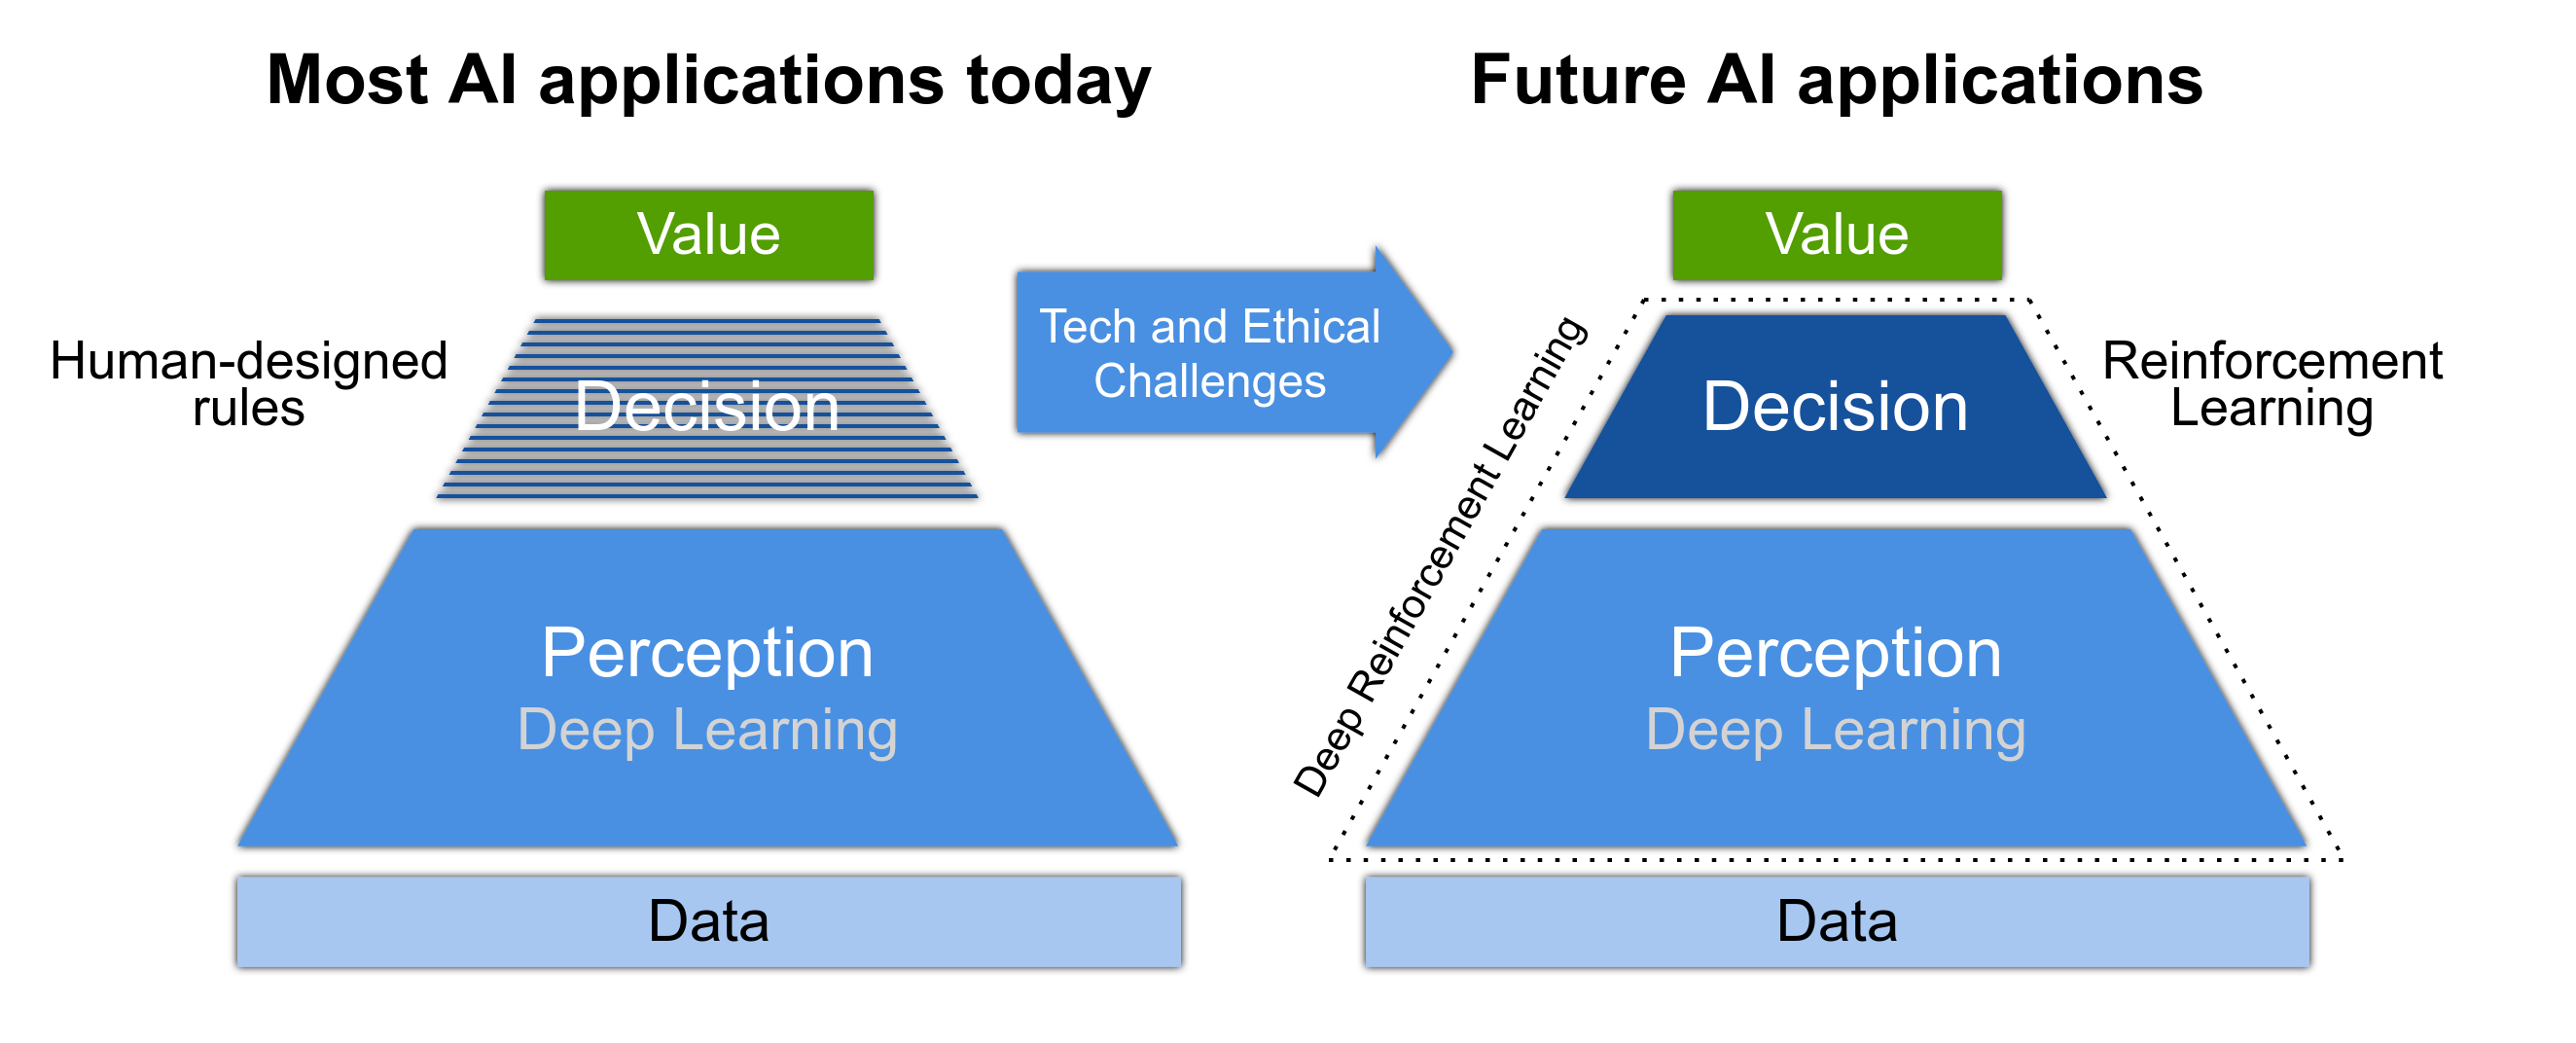
\includegraphics[width=\textwidth]{img/reinforcement-learning.png}
	\caption[Future transition in AI Applications]{Most AI applications today exploit deep learning and machine learning for image detection and computer vision. Decisions are made by optimal control algorithms which are hard-coded and designed by humans. The reinforcement learning approach aims to inject machine learning algorithms in the decision component of the algorithm to make steps towards Artificial General Intelligence (AGI) \cite{chara2018wild}.}
	\label{fig:futureai}
\end{figure}

Between the end of 2018 and the beginning of 2019, UC Berkeley and Google developed jointly a state-of-the-art off-policy model-free reinforcement learning algorithm called soft actor-critic (SAC) (see \vref{sac}). The critical goal is to provide a deep RL algorithm suitable for real-world problems and the related new challenges that they pose.
They outlined the desired properties of the ideal deep reinforcement learning algorithm:
\begin{description}
	\item[Sample Efficiency:] the process of learning in the real world can be a very time-consuming task. For this reason, it is desirable a functional sample complexity to learn skills successfully.
	\item[No sensitive hyperparameters:] as mentioned before, hyperparameter tuning could be a tough task to complete in real-world experiments as it could require numerous repetitions in situations where the cost in terms of time and money could be burdensome. The proposed solution of the authors is maximum entropy RL which provides a robust framework that minimises the need for hyperparameter tuning.
	\item[Off-policy learning:] this learning approach allows the reuse of collected data for various tasks. This possibility helps the process of prototyping a new task when adjusting parameters or choosing a different reward function.
\end{description}

Soft actor-critic (SAC) represents a deep RL algorithm capable of satisfying the previously mentioned requirements. The authors of \cite{haarnoja2018soft,haarnoja2018alg} revealed that the algorithm is capable of solving real-world robotic tasks in a conspicuous but acceptable number of hours, showing its robustness to hyperparameters and working on a large variety of simulated environments always using the same set of parameters.
Not only it shows great performances in numerous challenging tasks compared to deep deterministic policy gradient (DDPG), twin delayed deep deterministic policy gradient (TD3) \cite{fujimoto2018addressing} and proximal policy optimisation (PPO) \cite{schulman2017proximal}, but reveals its power by solving three tasks from scratch without relying on simulators or demonstrations \cite{bair2019soft}.

The real-world robotic task involving a 3-finger dexterous robotic hand to manipulate an object similar to a sink faucet with a coloured end presented in \cite[Section 7.3]{haarnoja2018alg} shows similar concepts to the task analysed in this thesis for what concerns the framework of deep reinforcement learning exploited. The algorithm exploits raw RGB images and processes them through a convolutional neural network. The final goal of the robot is to rotate the valve into the correct position -- with the coloured part pointing to the right -- starting from a random position for each episode. The results obtained represents one of the most sophisticated real-world robotic manipulation tasks learned end-to-end with deep reinforcement learning, starting from raw images and without any previous simulation or pretraining phase.

Taking all arguments into account, we decided to follow \cite{kendall2019learning} implementing a similar self-driving framework based on the design of a control system for a small toy robot called Anki Cozmo (see \vref{ch:ch4}). Therefore, we formalise the autonomous driving learning problem as a Markov decision process to enable the application of reinforcement learning algorithms, taking into account the improvements mentioned in this section about model-free reinforcement learning algorithms applied to real-world robotic problems. \Vref{ch:ch4} provides a detailed description of the choice made and the system design. \Vref{ch:ch5} reports the experiment we carried out in the environment we designed.







